\section*{Experiment No.2}
\subsection*{First series of measurements}
\begin{figure}[h]
\begin{center}
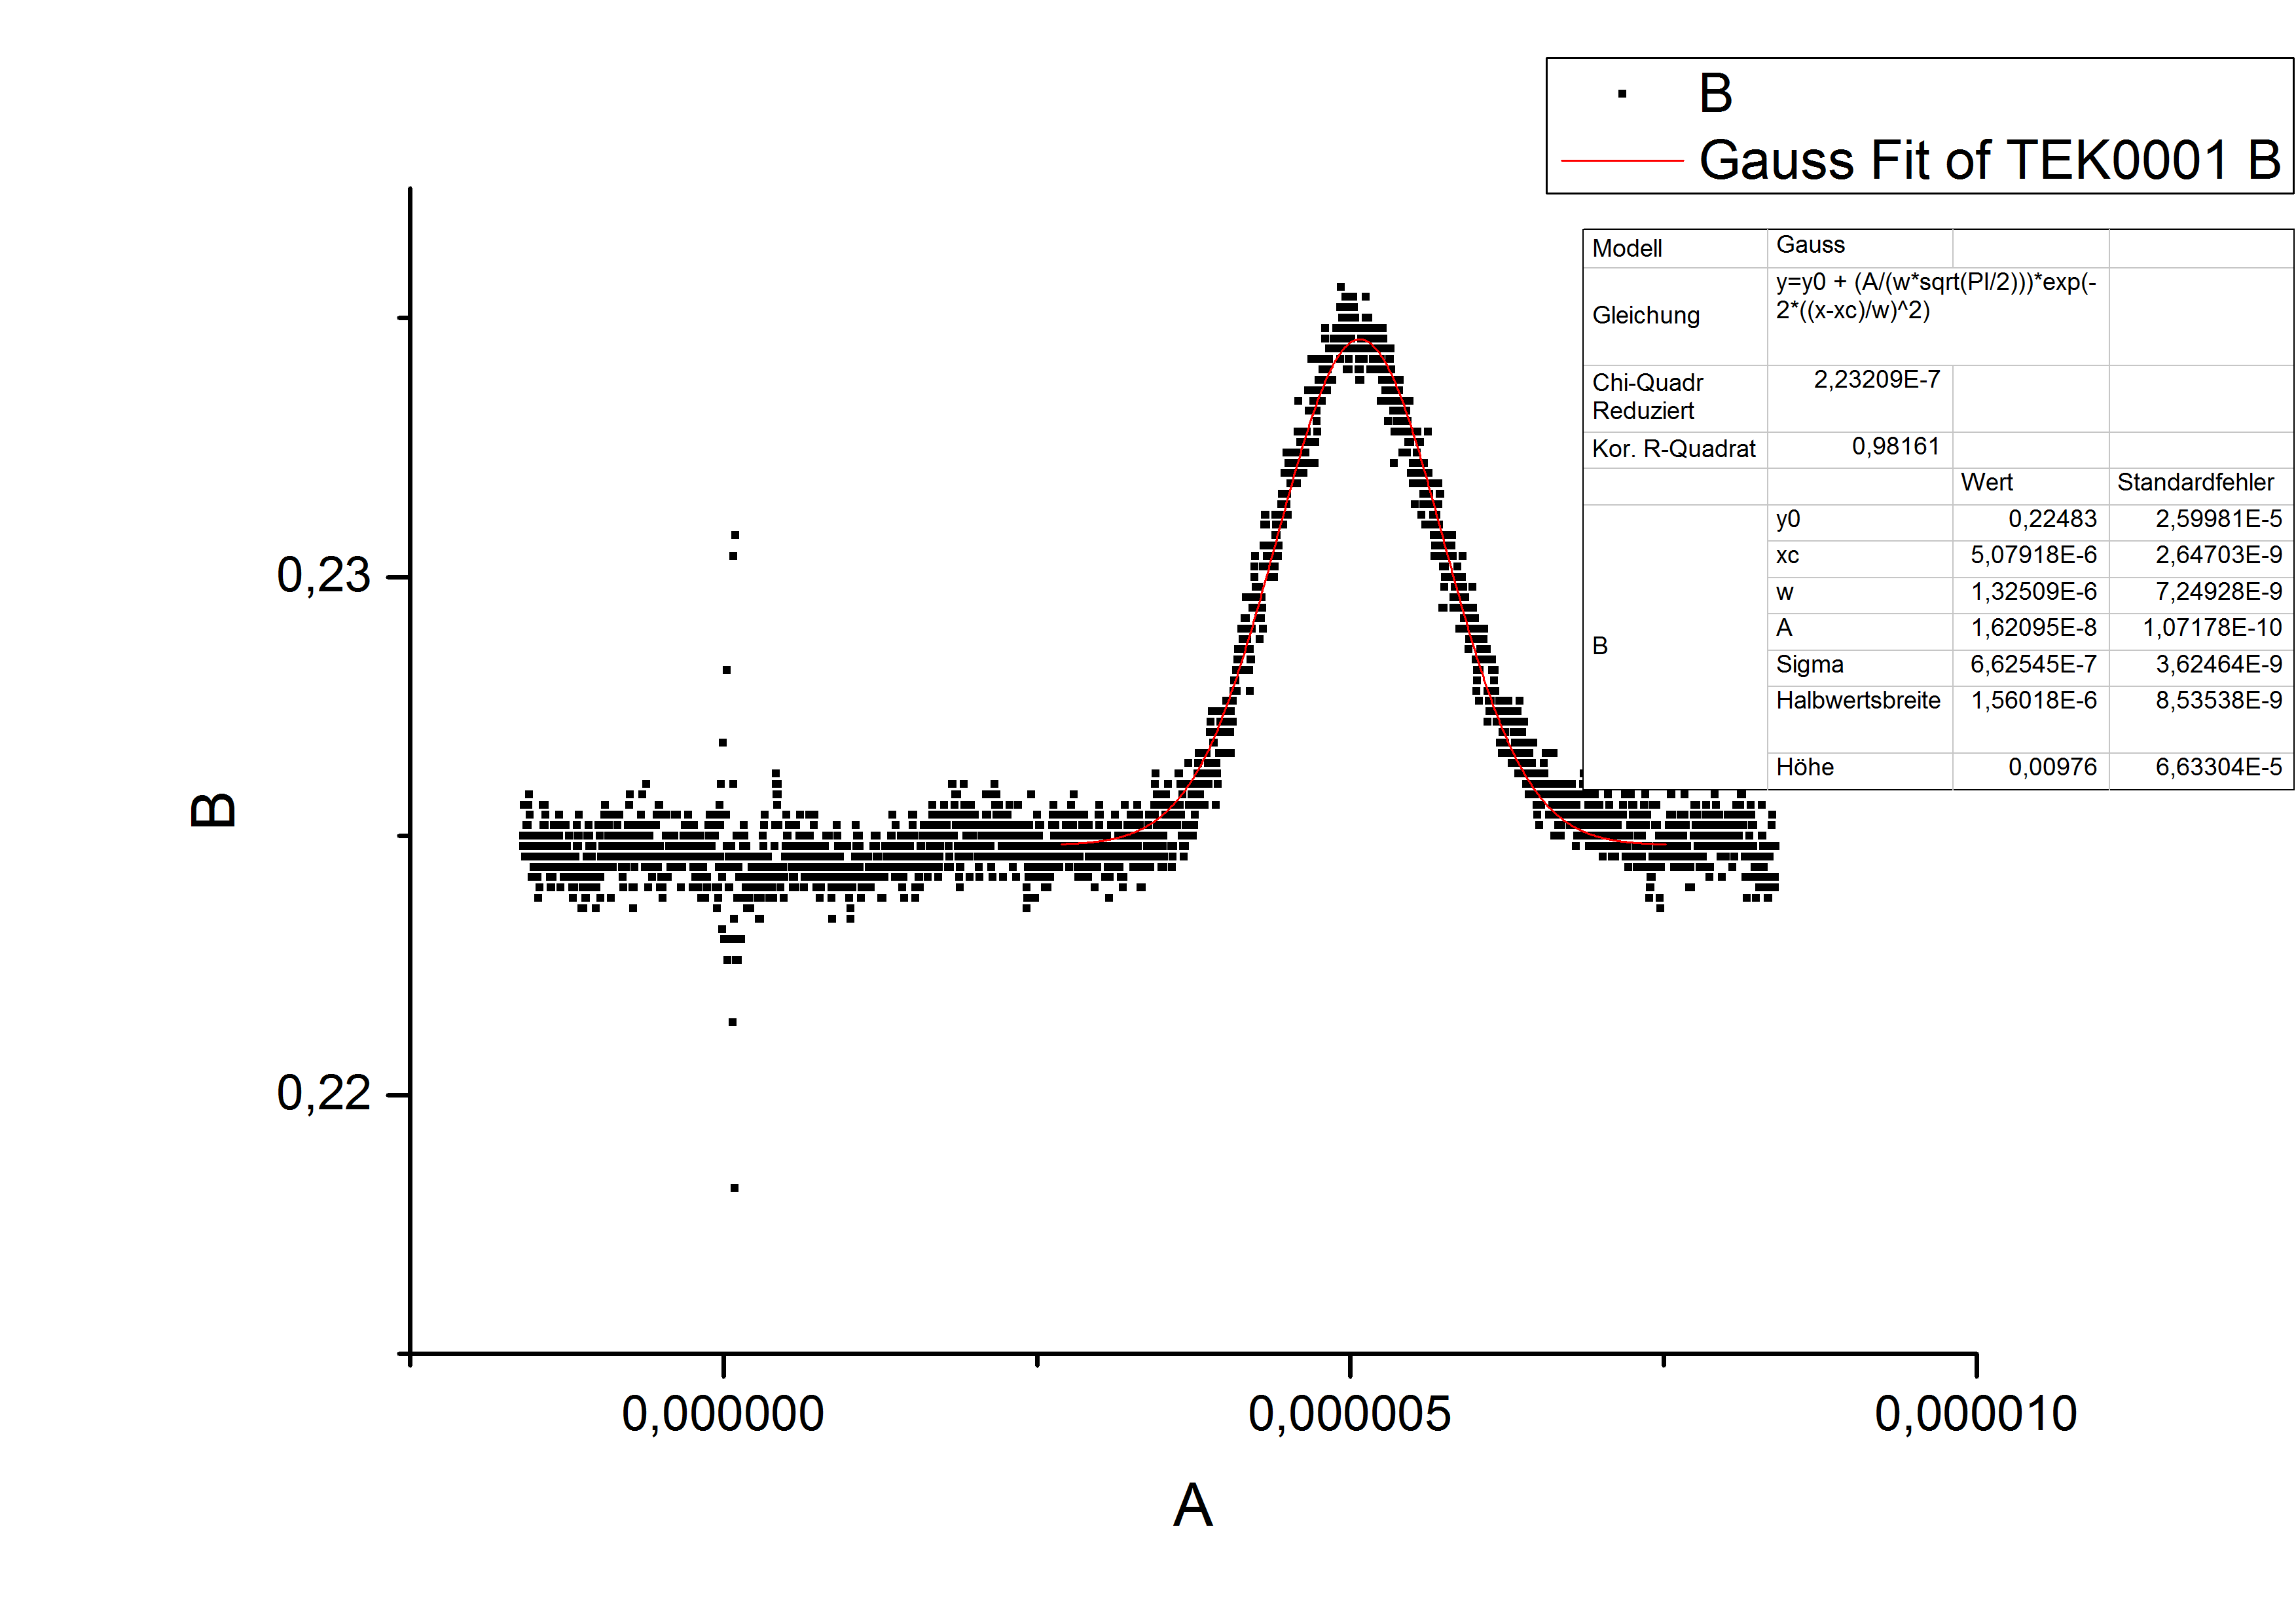
\includegraphics[scale=0.25]{Bilder/Teil2/Graph1}
\caption{Graph at 2.52mm.}
\label{fig:graph1}
\end{center}
\end{figure}
\begin{figure}[h]
\begin{center}
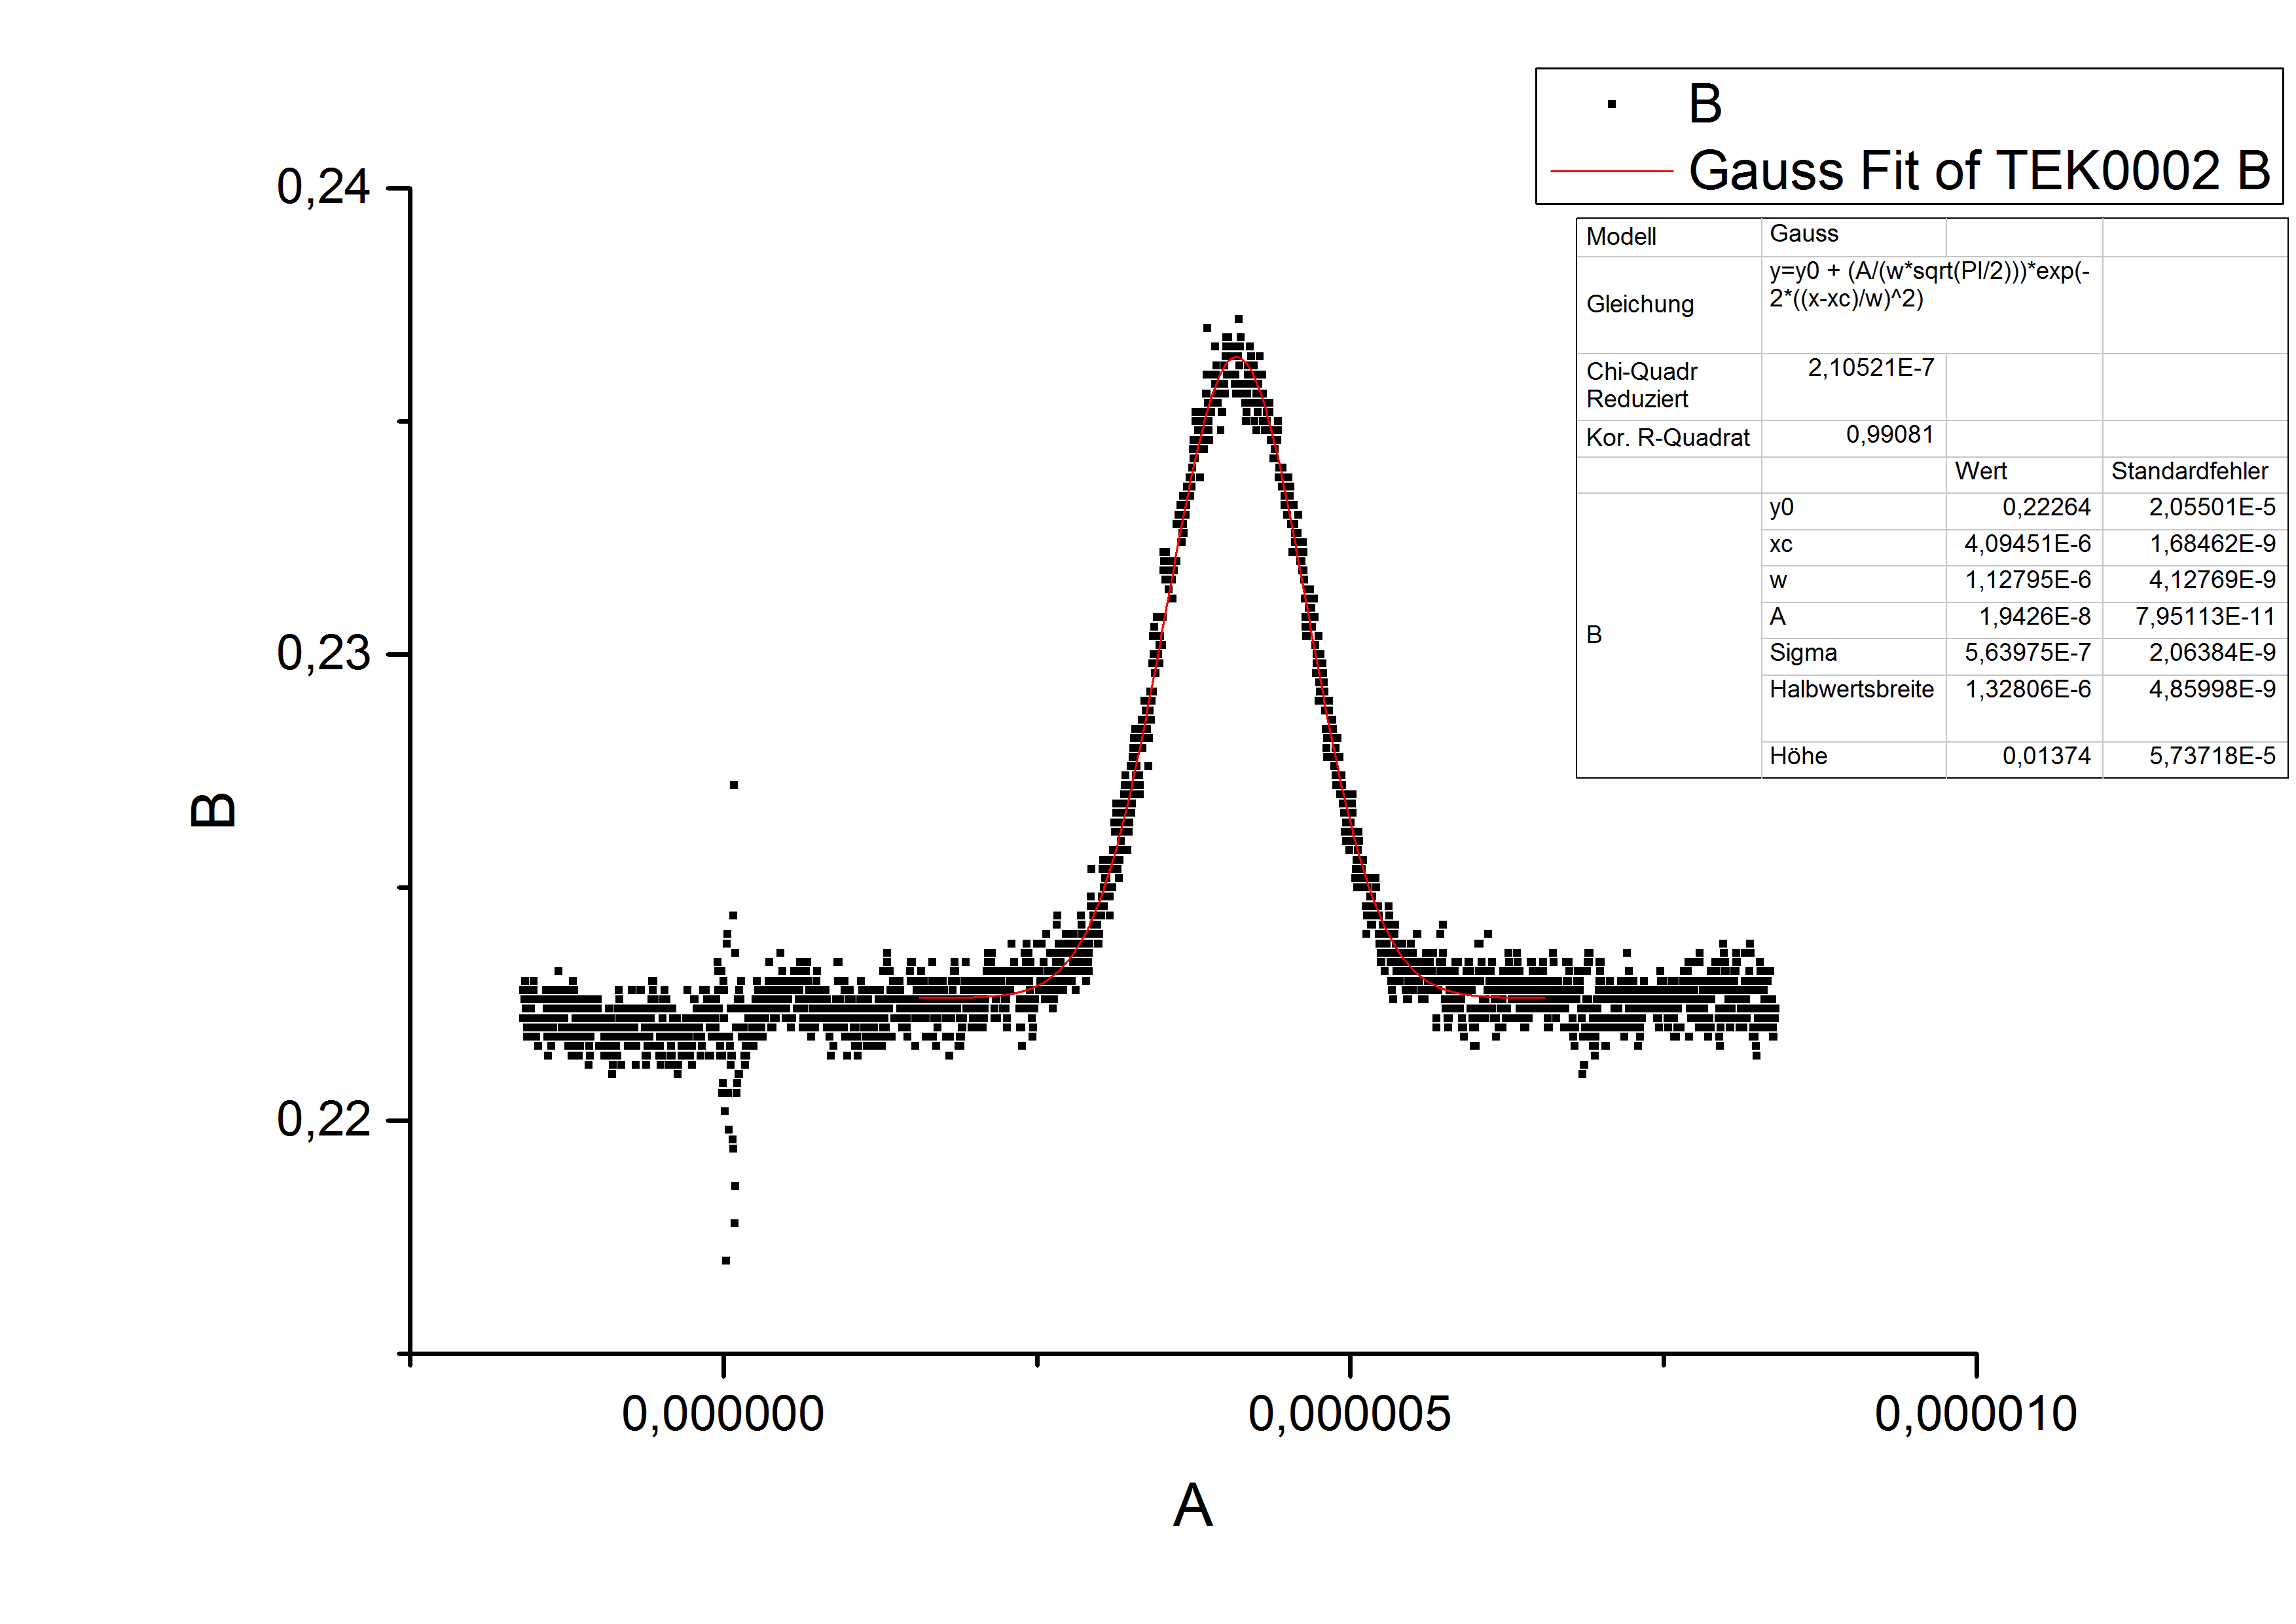
\includegraphics[scale=0.25]{Bilder/Teil2/Graph2}
\caption{Graph at 1.99mm.}
\label{fig:graph2}
\end{center}
\end{figure}
\begin{figure}[h]
\begin{center}
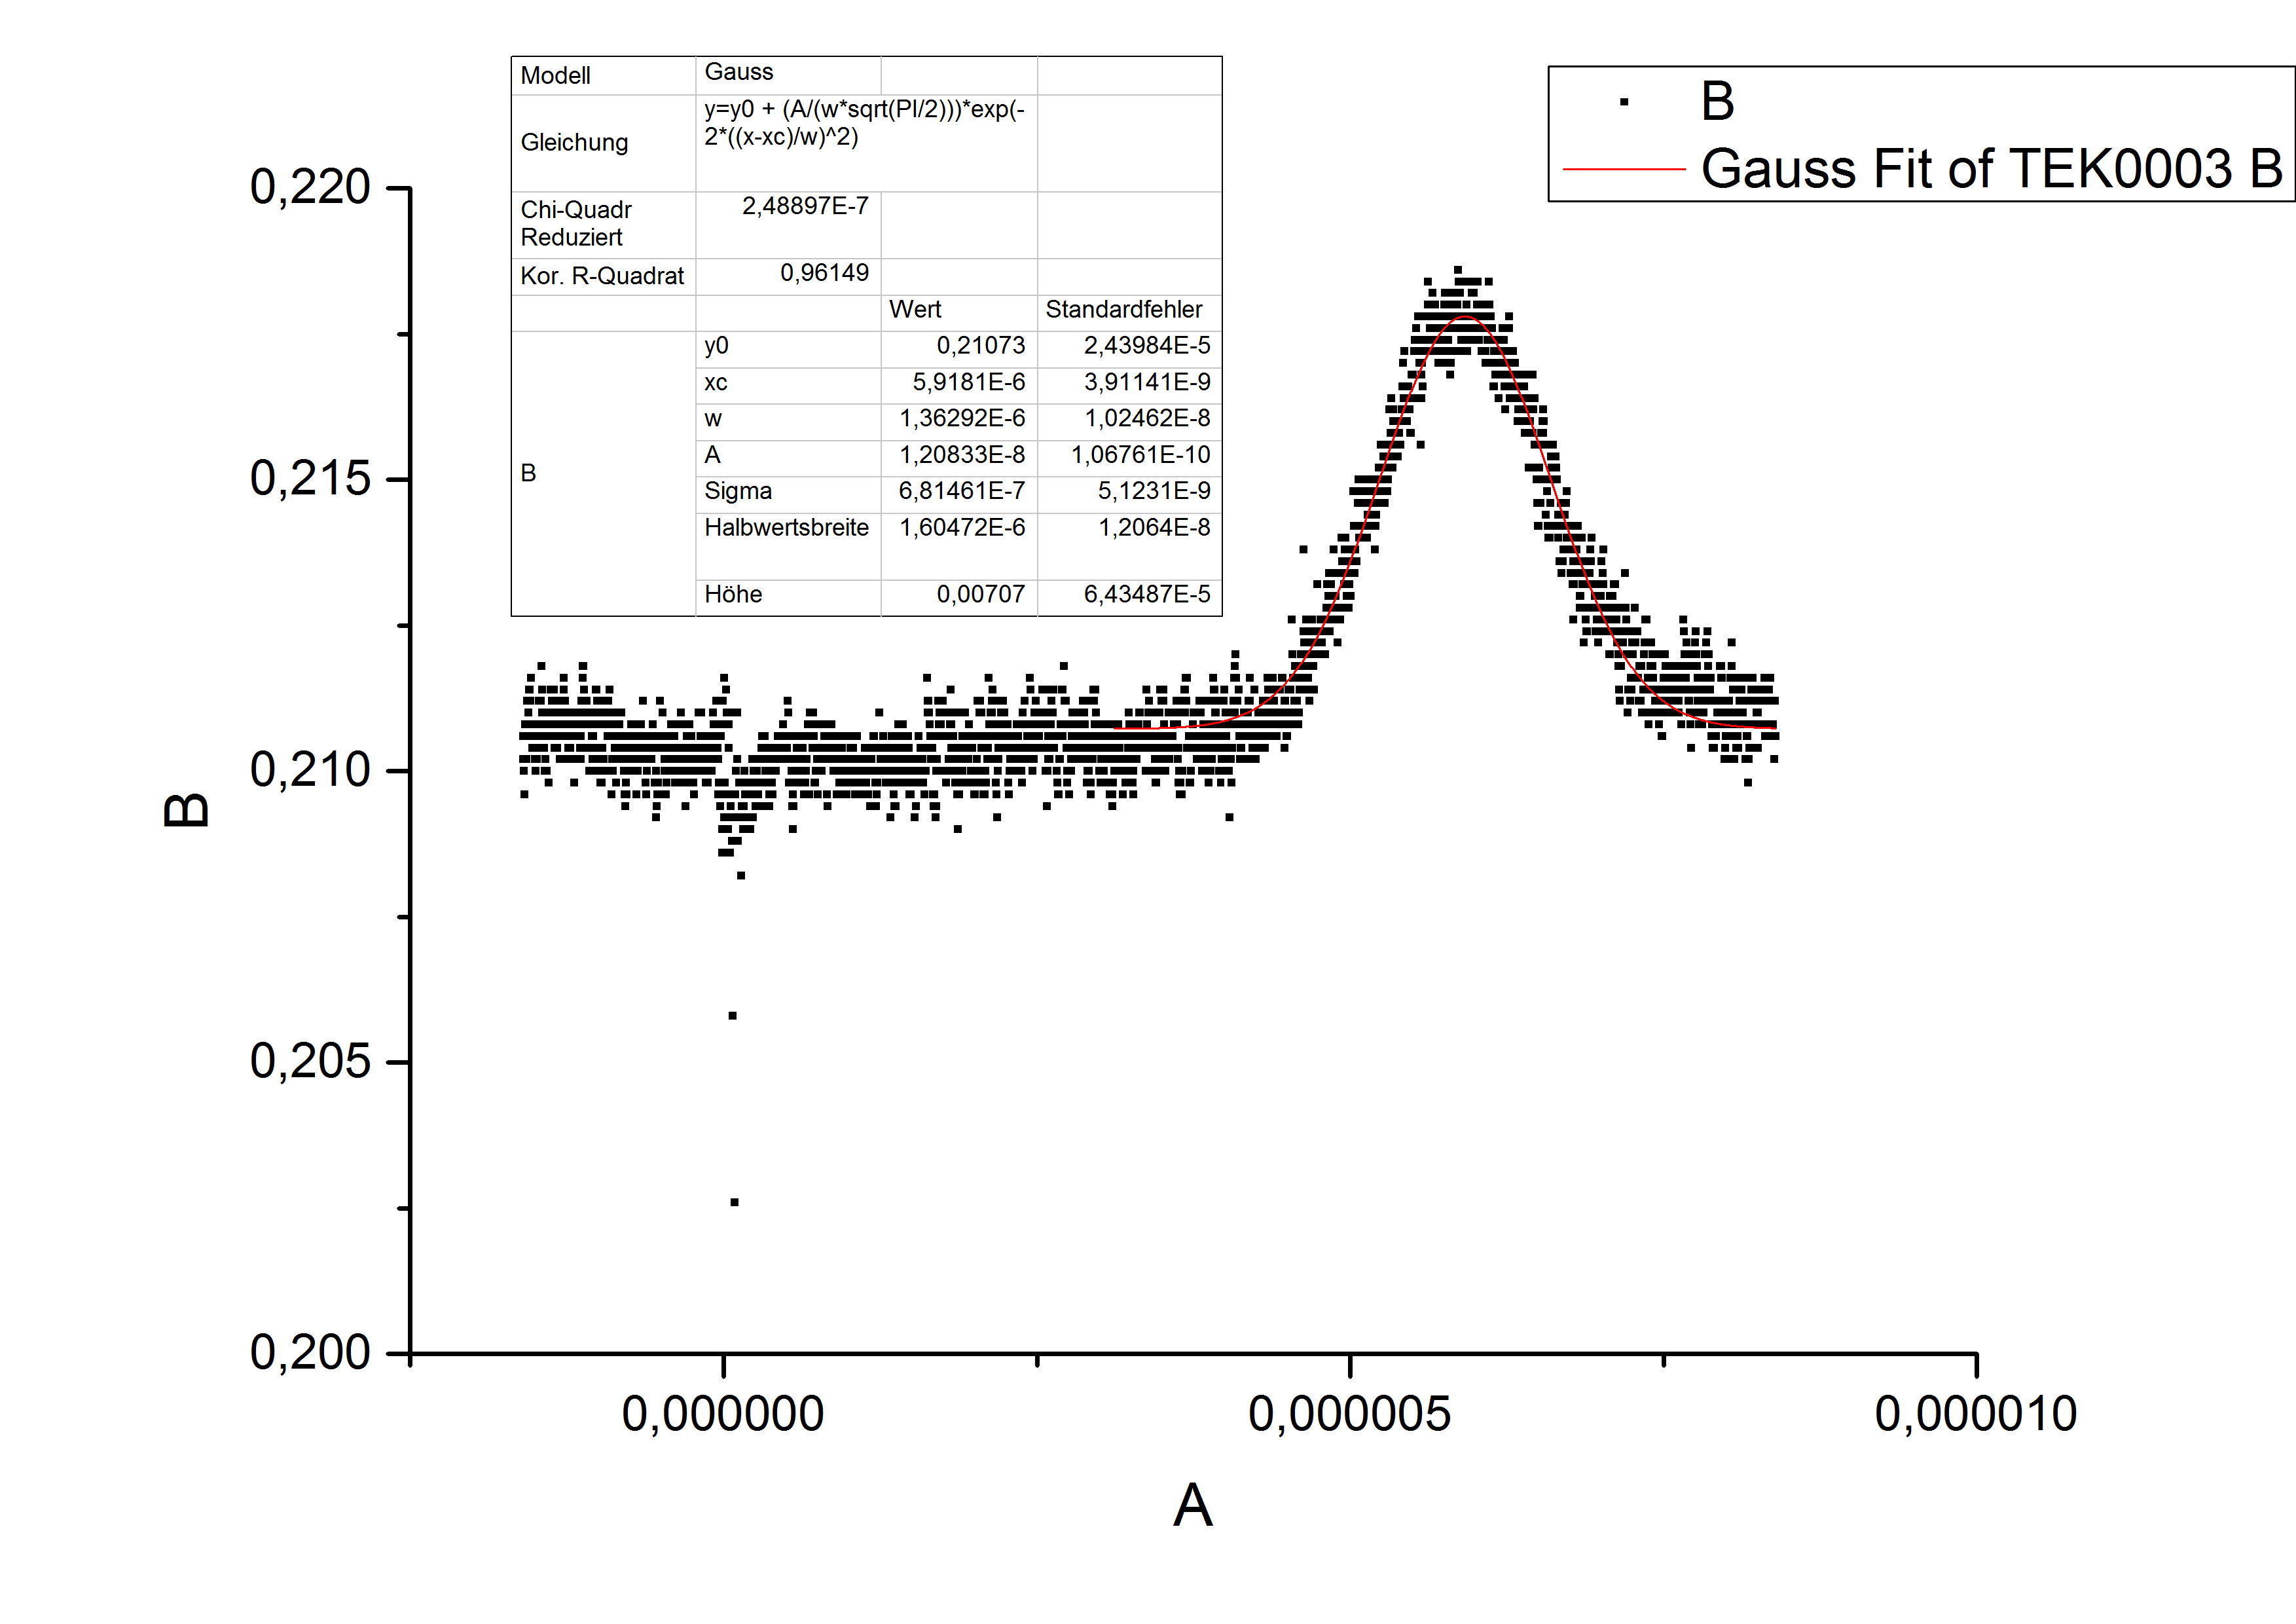
\includegraphics[scale=0.25]{Bilder/Teil2/Graph3}
\caption{Graph at 3.01mm.}
\label{fig:graph3}
\end{center}
\end{figure}
\begin{figure}[h]
\begin{center}
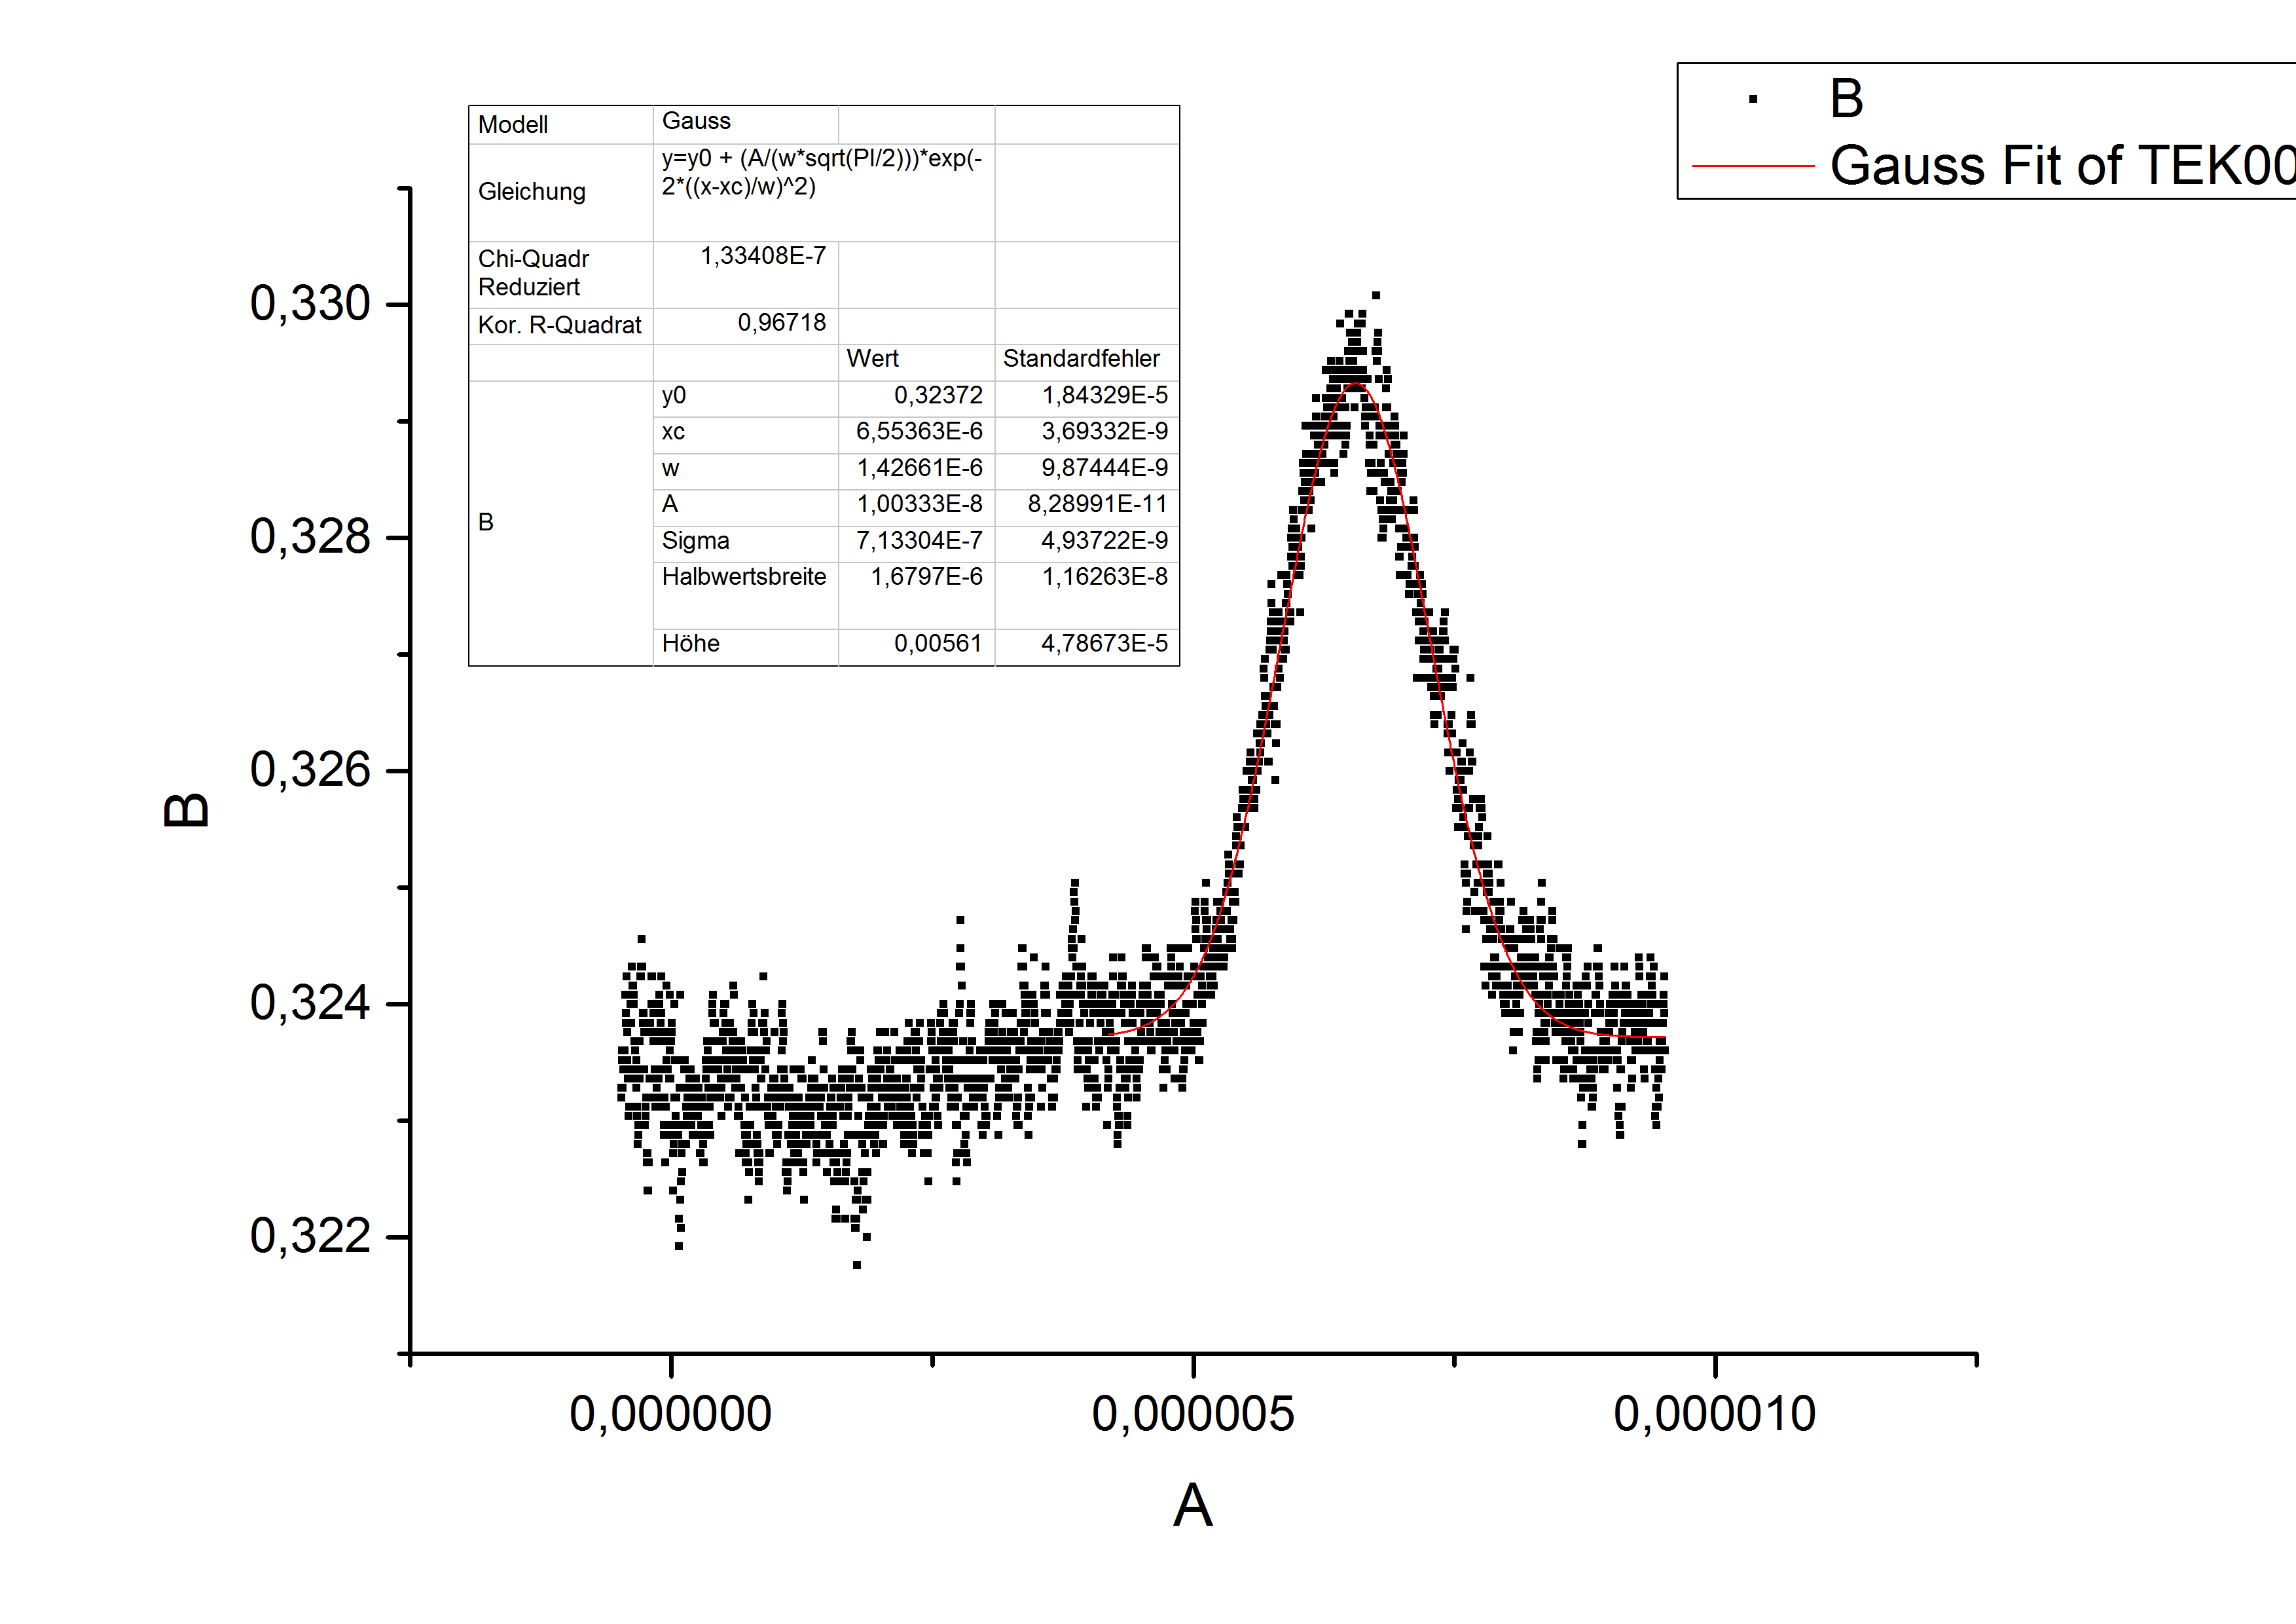
\includegraphics[scale=0.25]{Bilder/Teil2/Graph4}
\caption{Graph at 3.55mm.}
\label{fig:graph4}
\end{center}
\end{figure}
\begin{figure}[h]
\begin{center}
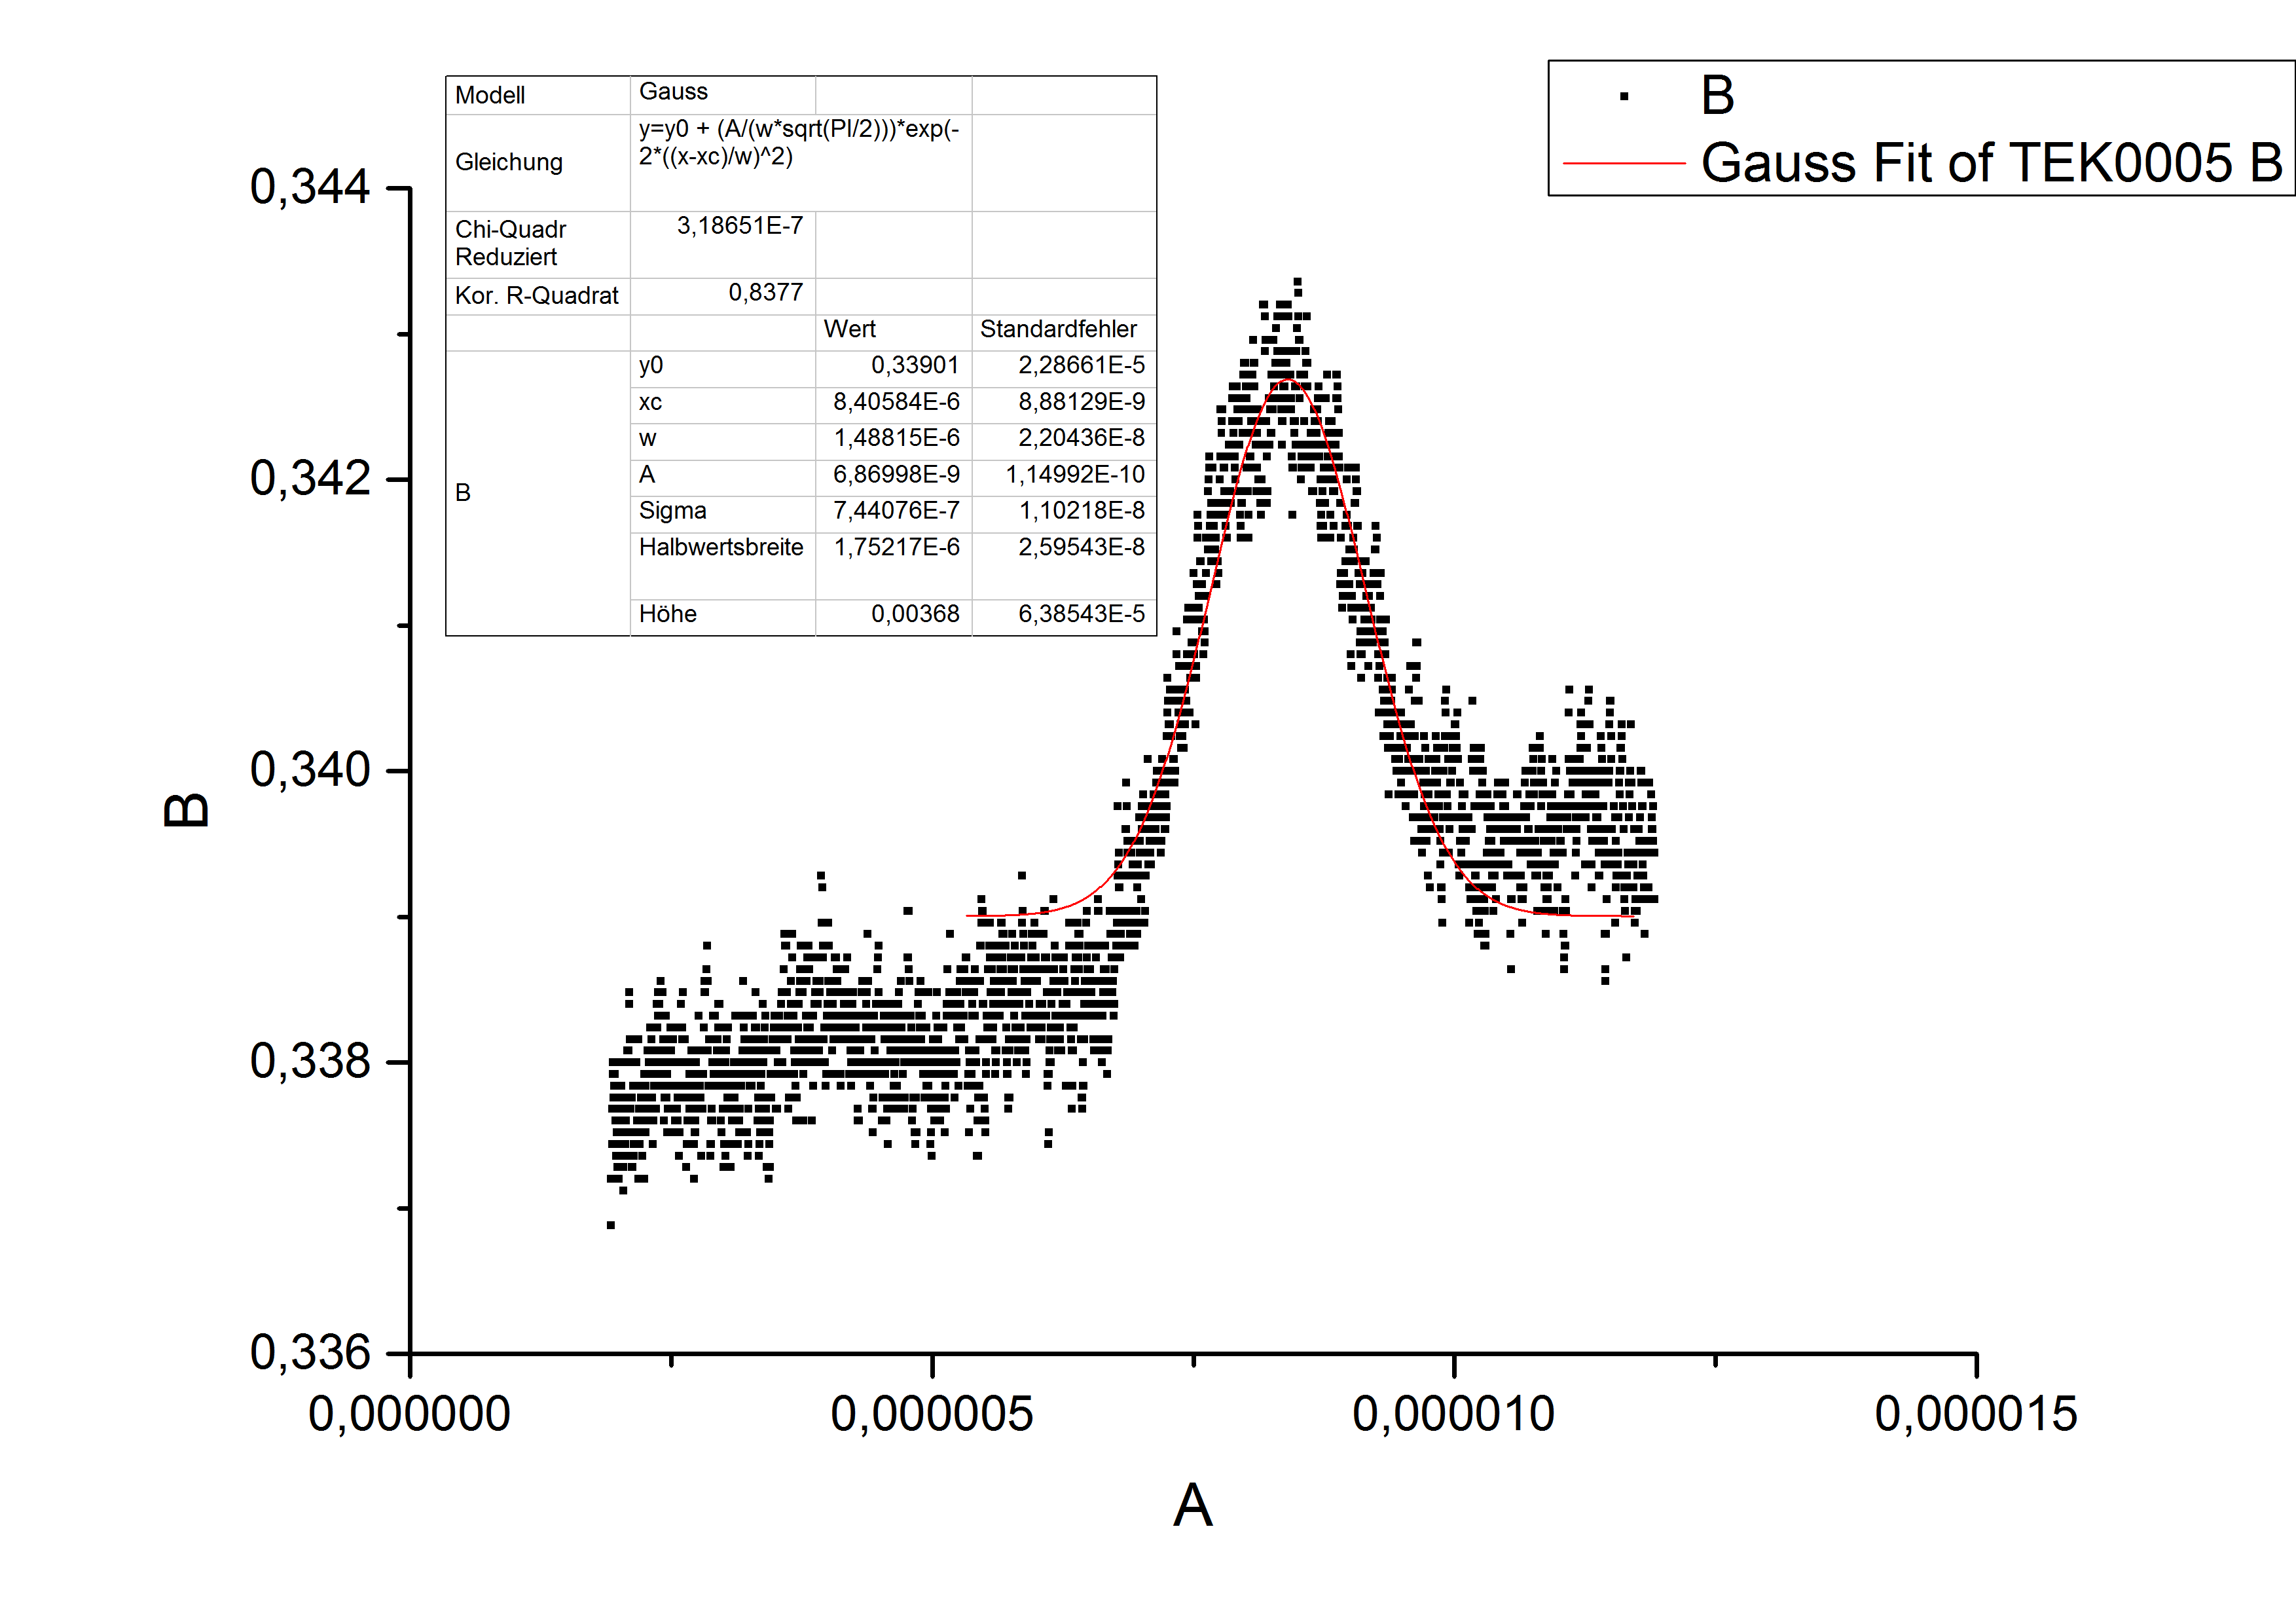
\includegraphics[scale=0.25]{Bilder/Teil2/Graph5}
\caption{Graph at 4.01mm.}
\label{fig:graph5}
\end{center}
\end{figure}
\begin{figure}[h]
\begin{center}
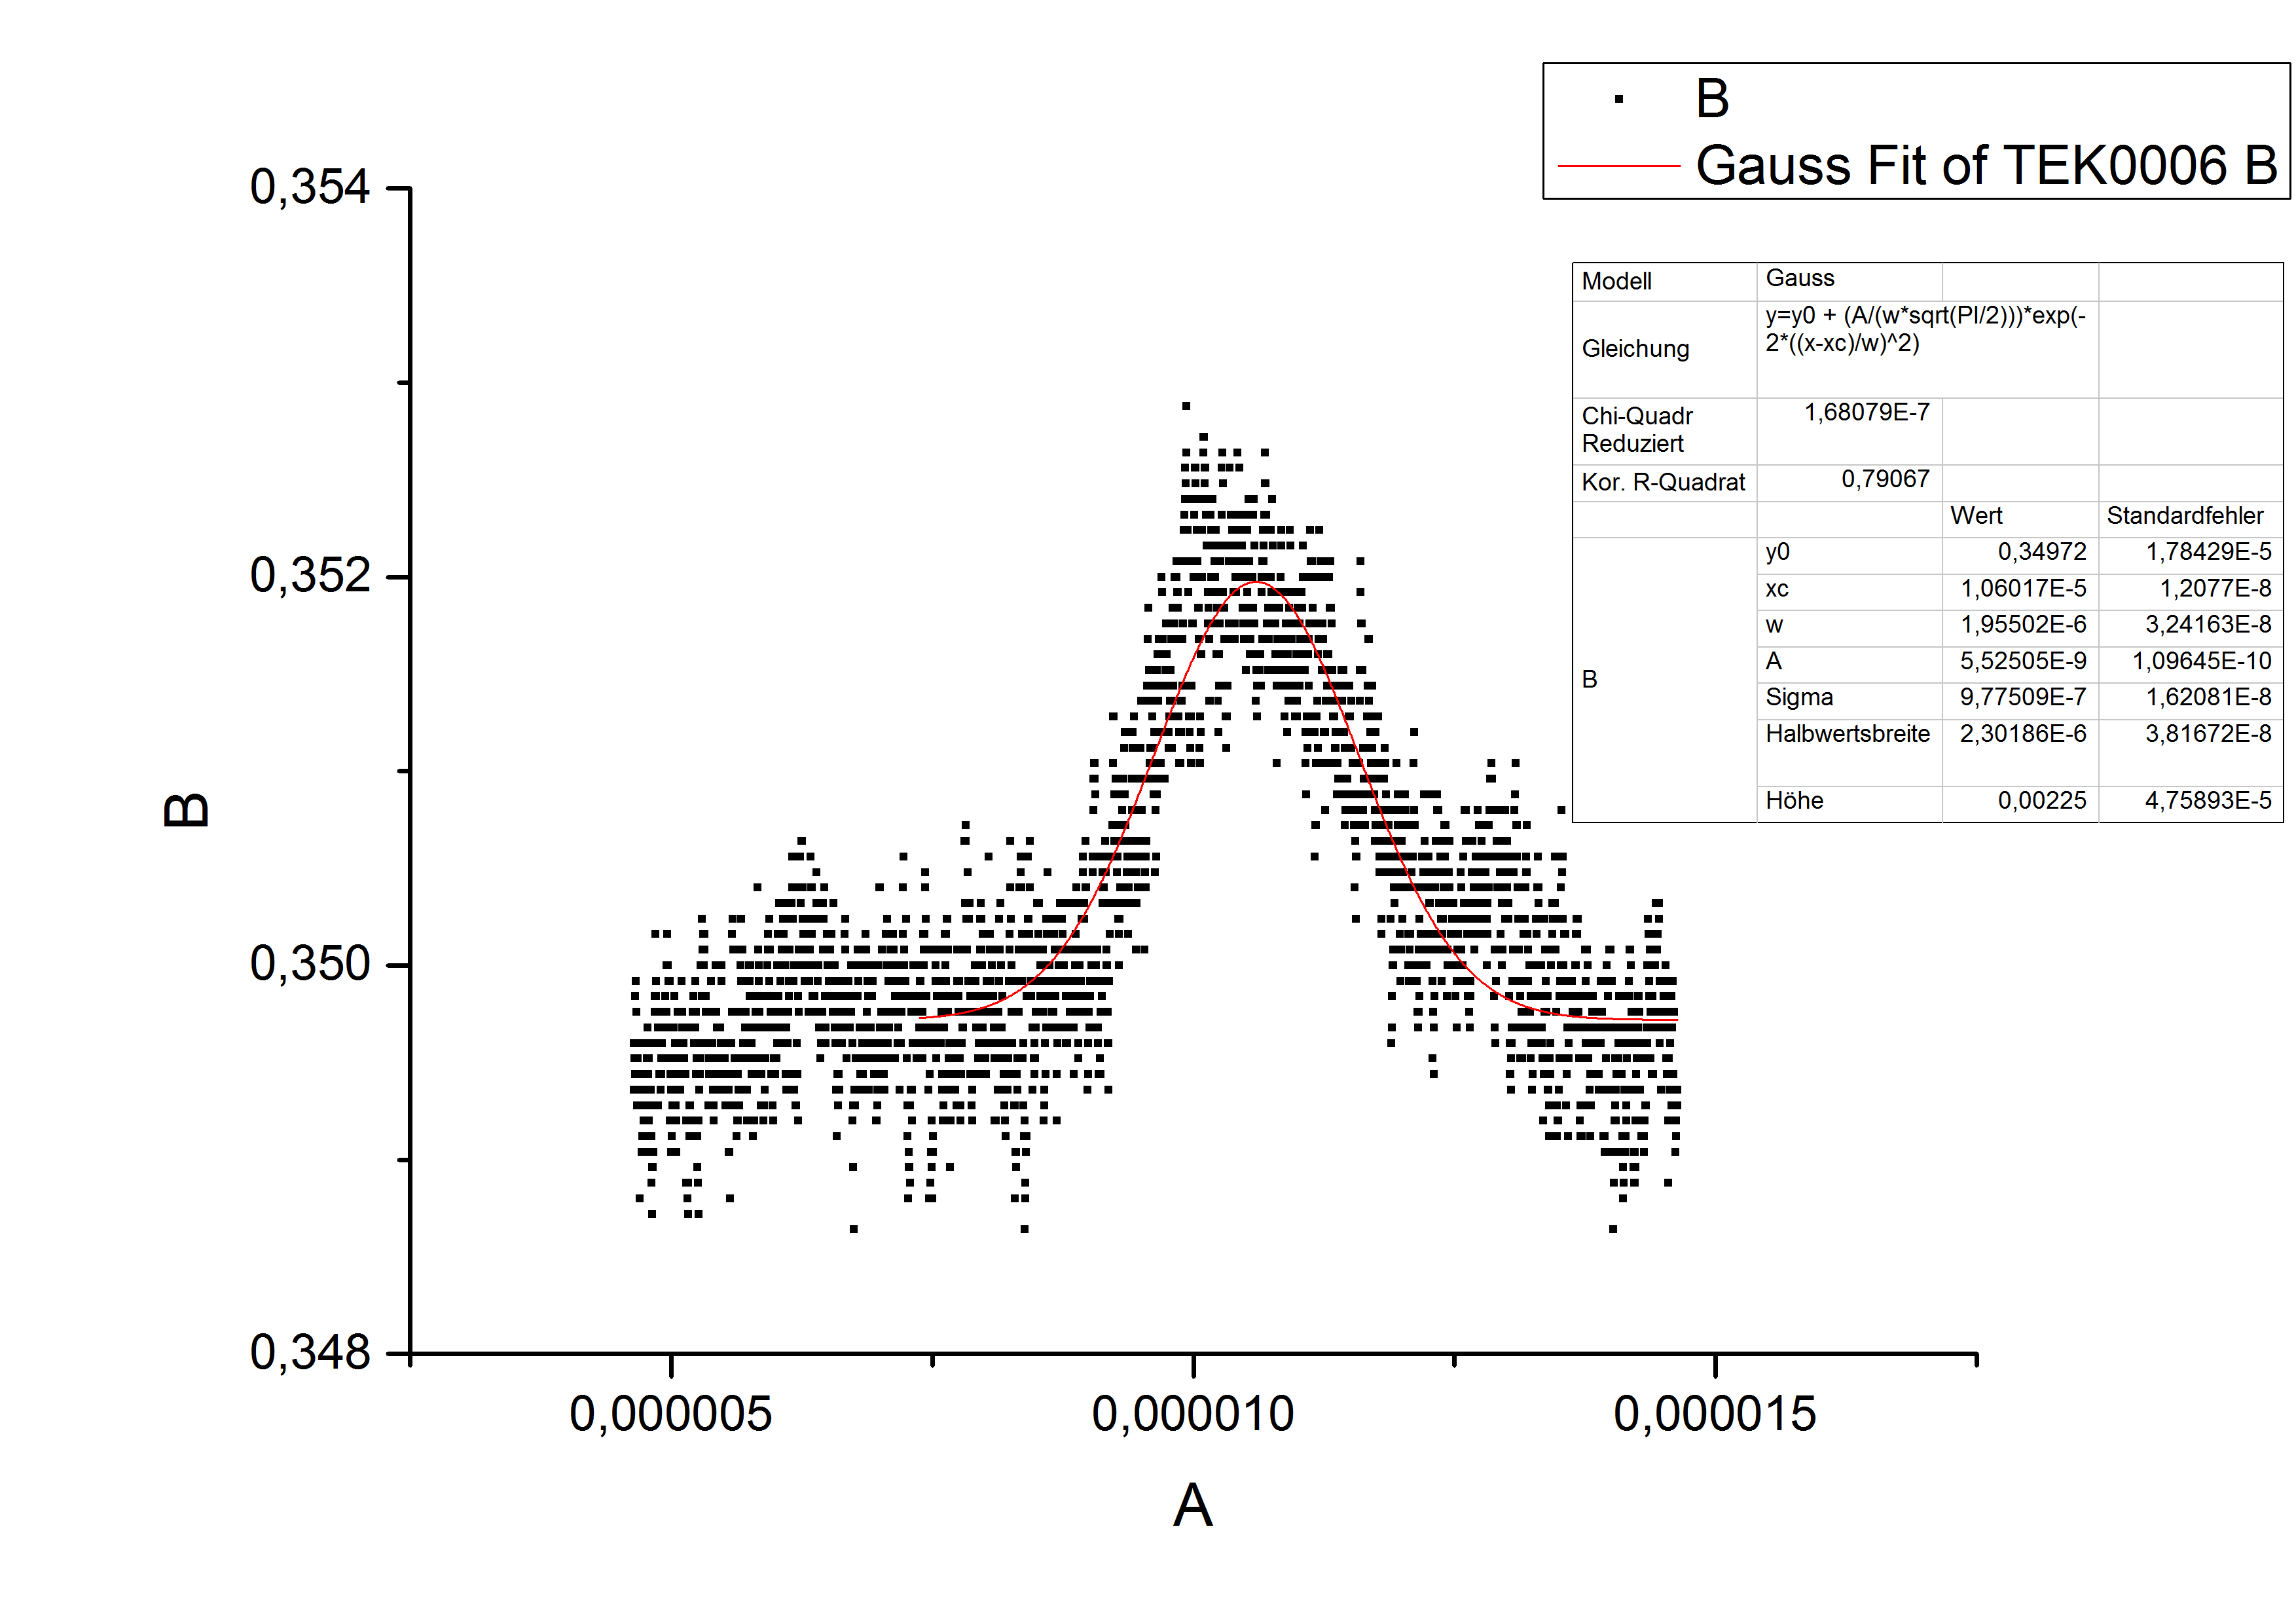
\includegraphics[scale=0.25]{Bilder/Teil2/Graph6}
\caption{Graph at 4.53mm.}
\label{fig:graph6}
\end{center}
\end{figure}
\begin{figure}[h]
\begin{center}
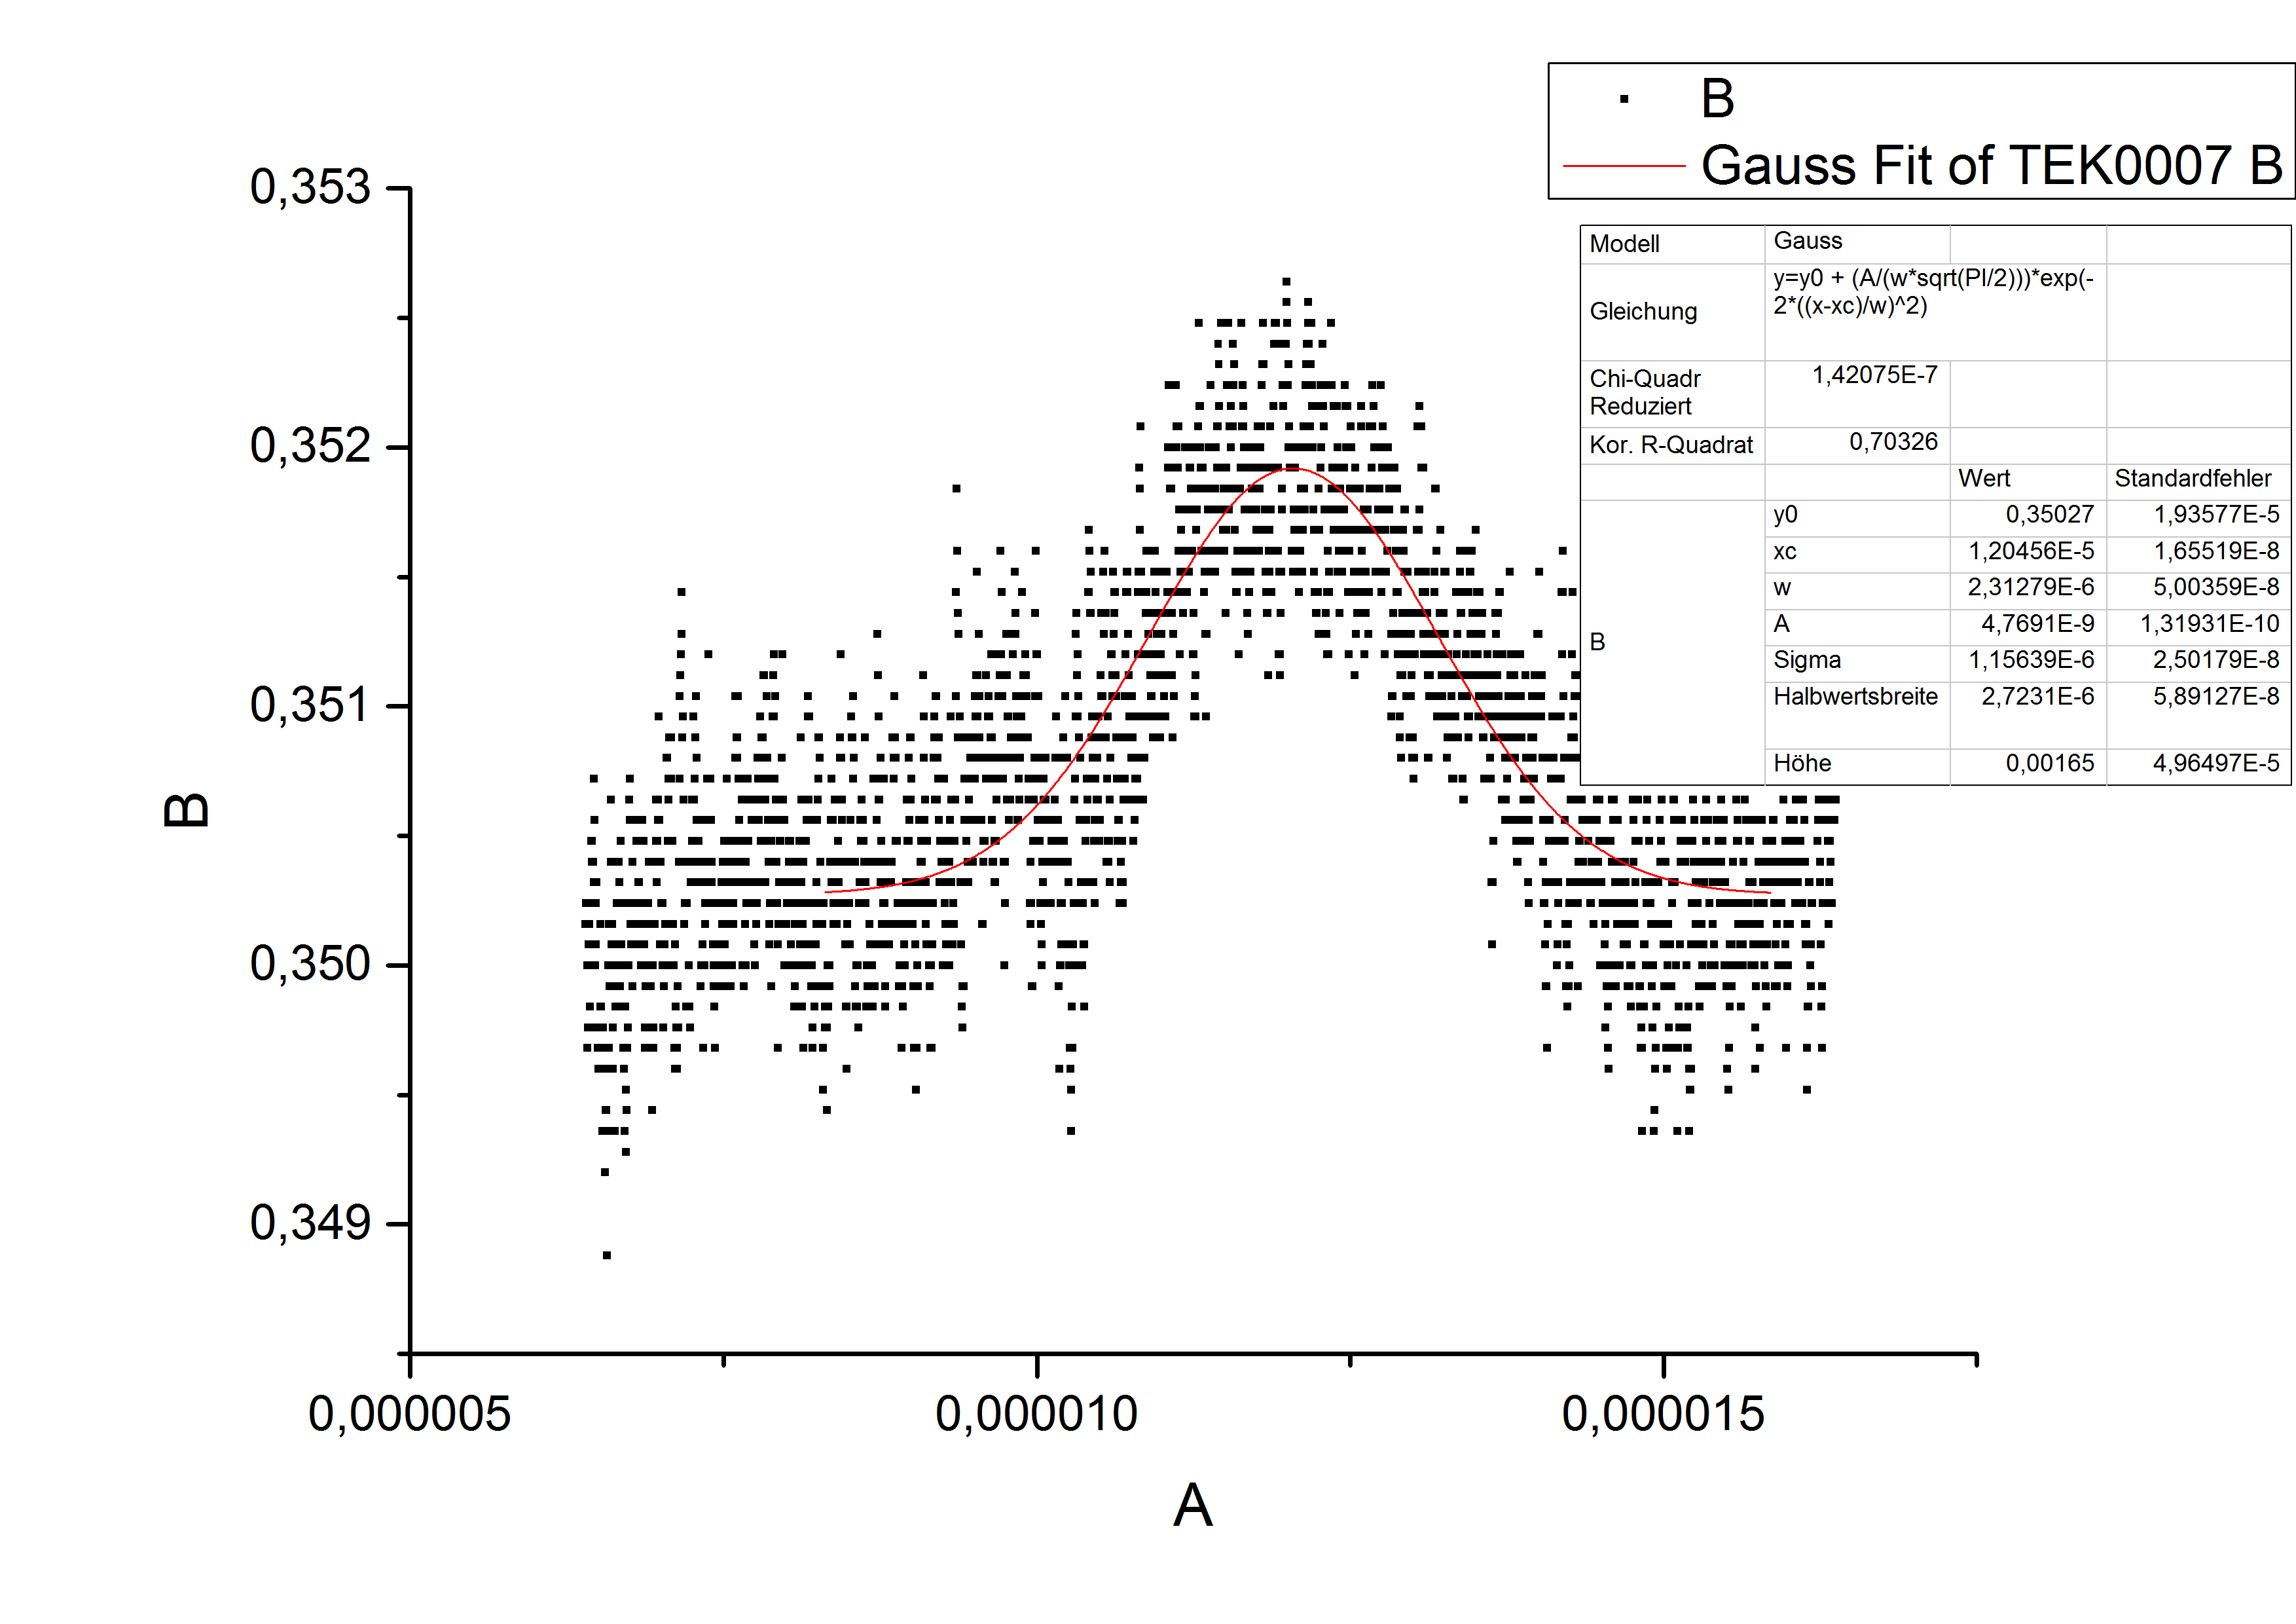
\includegraphics[scale=0.25]{Bilder/Teil2/Graph7}
\caption{Graph at 5.05mm.}
\label{fig:graph7}
\end{center}
\end{figure}
\begin{figure}[h]
\begin{center}
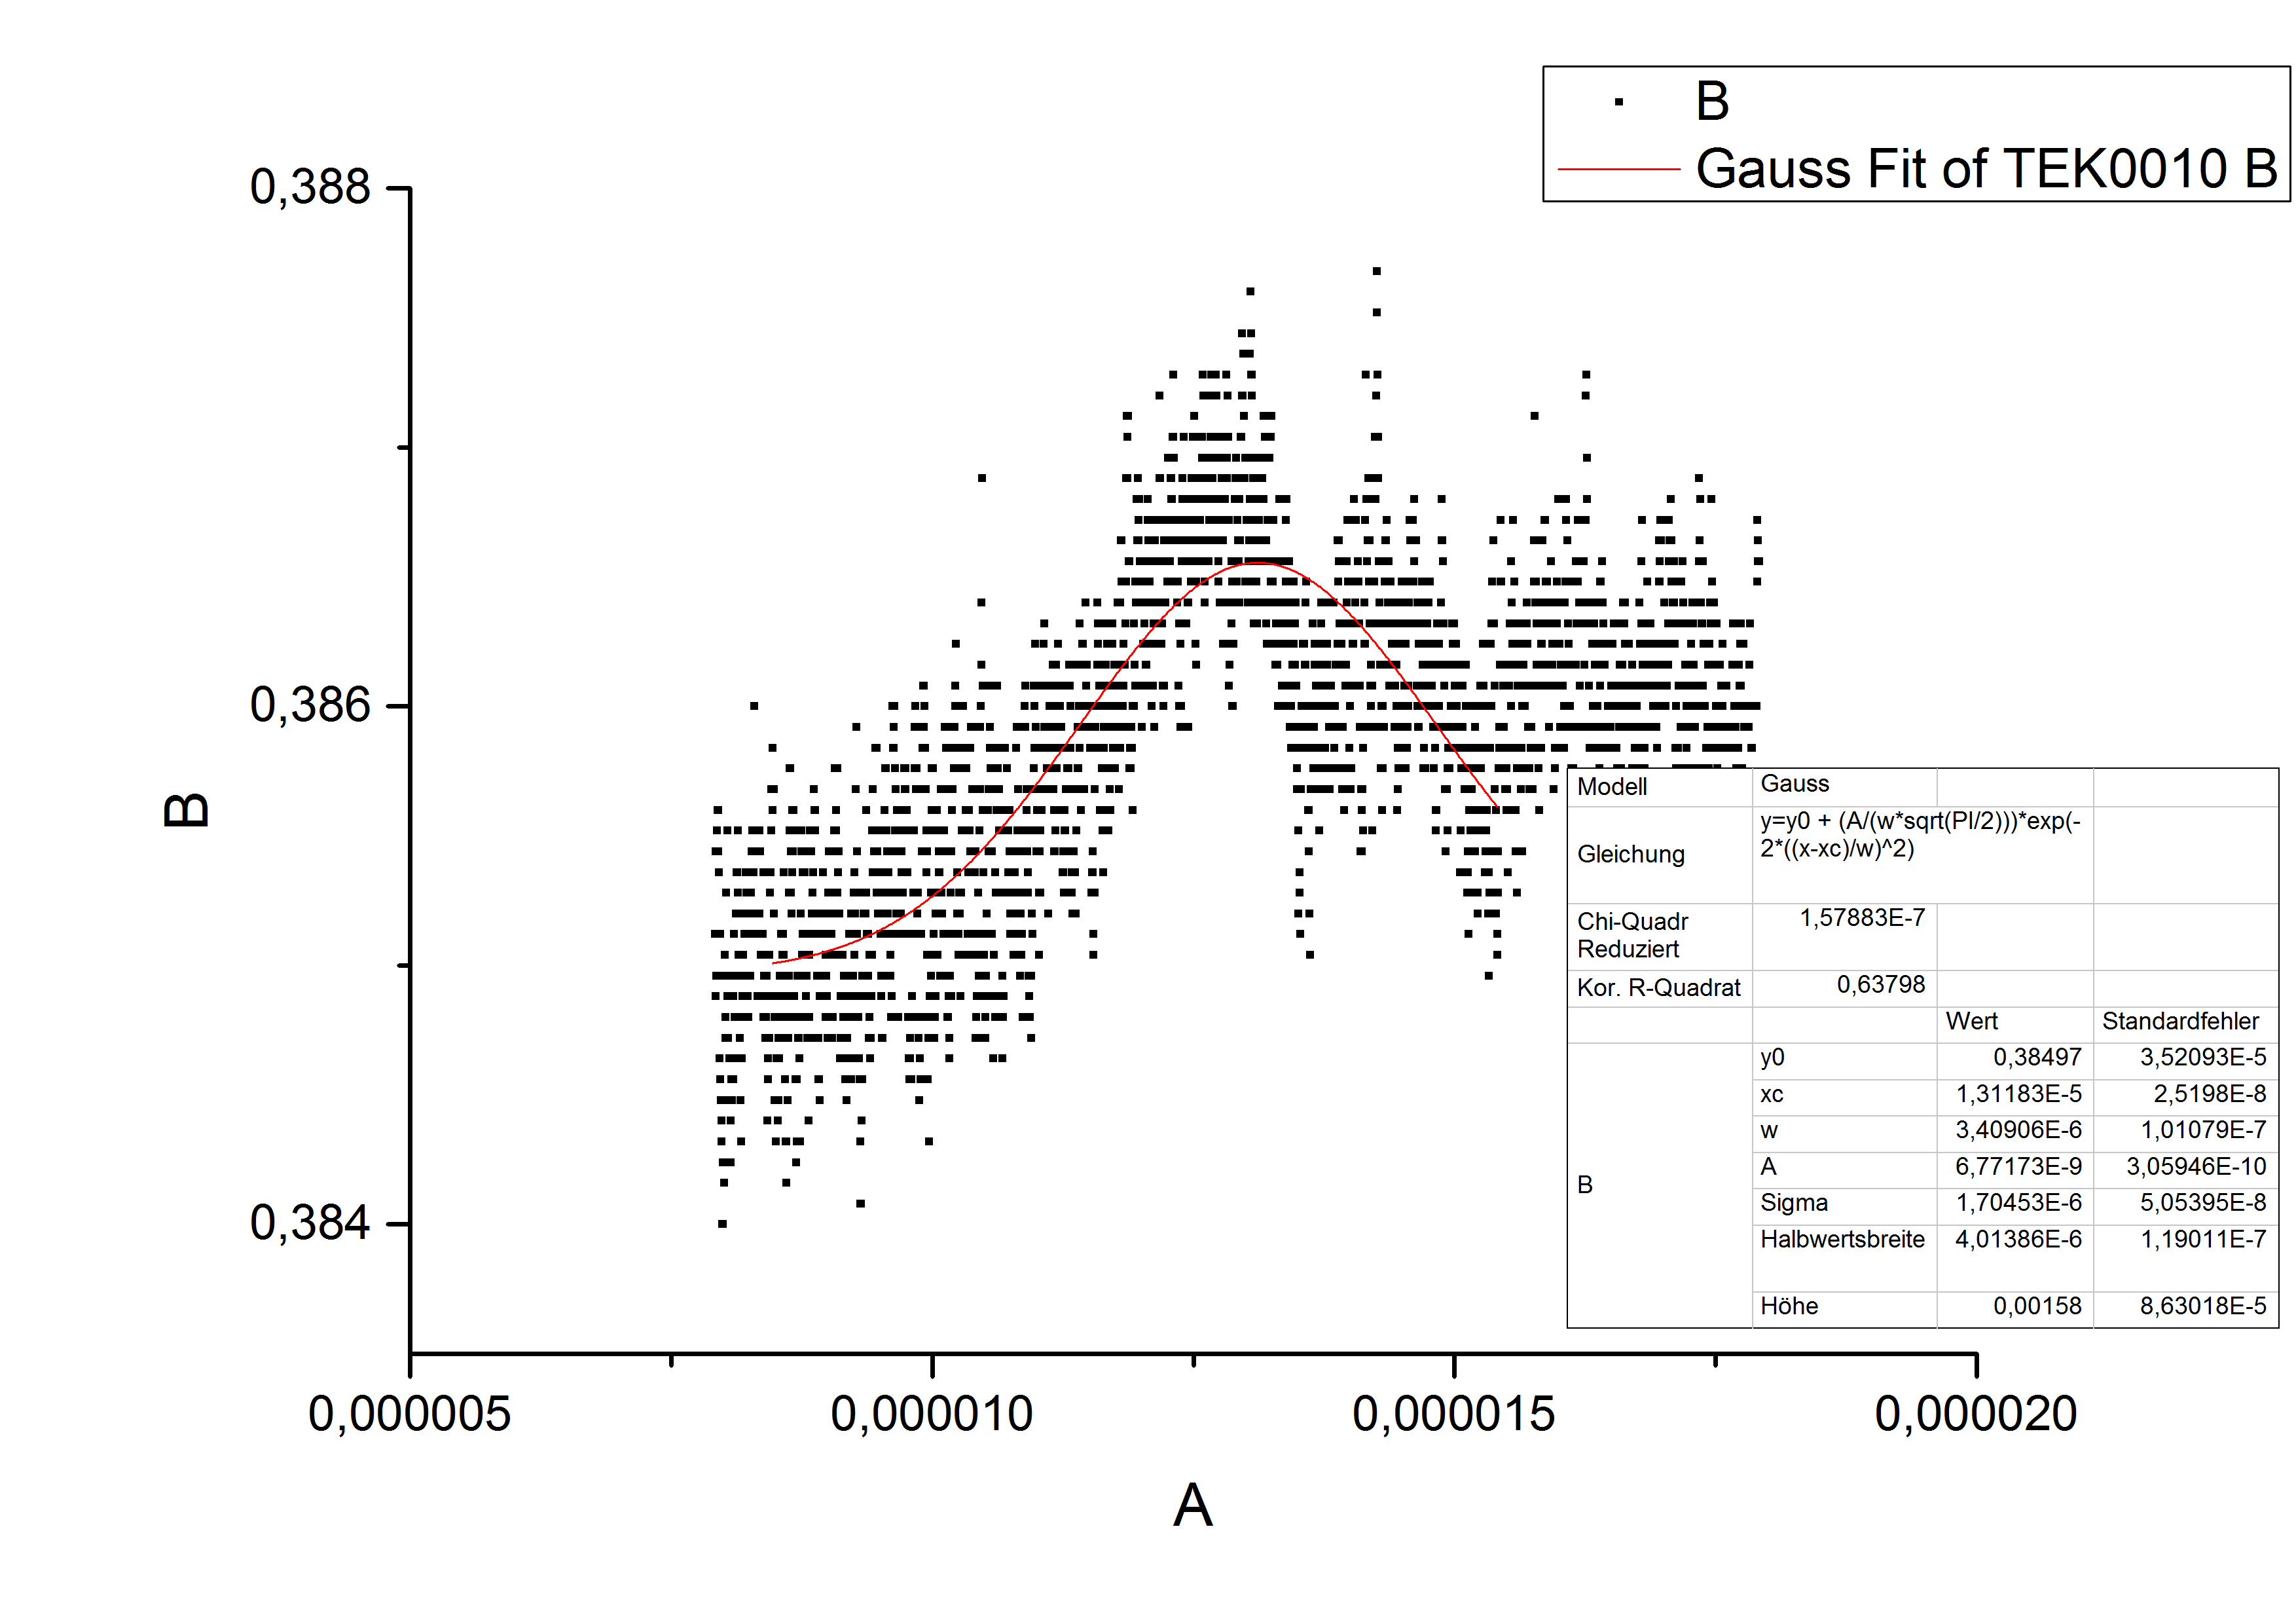
\includegraphics[scale=0.25]{Bilder/Teil2/Graph8}
\caption{Graph at 55.52mm.}
\label{fig:graph8}
\end{center}
\end{figure}
\begin{figure}[h]
\begin{center}
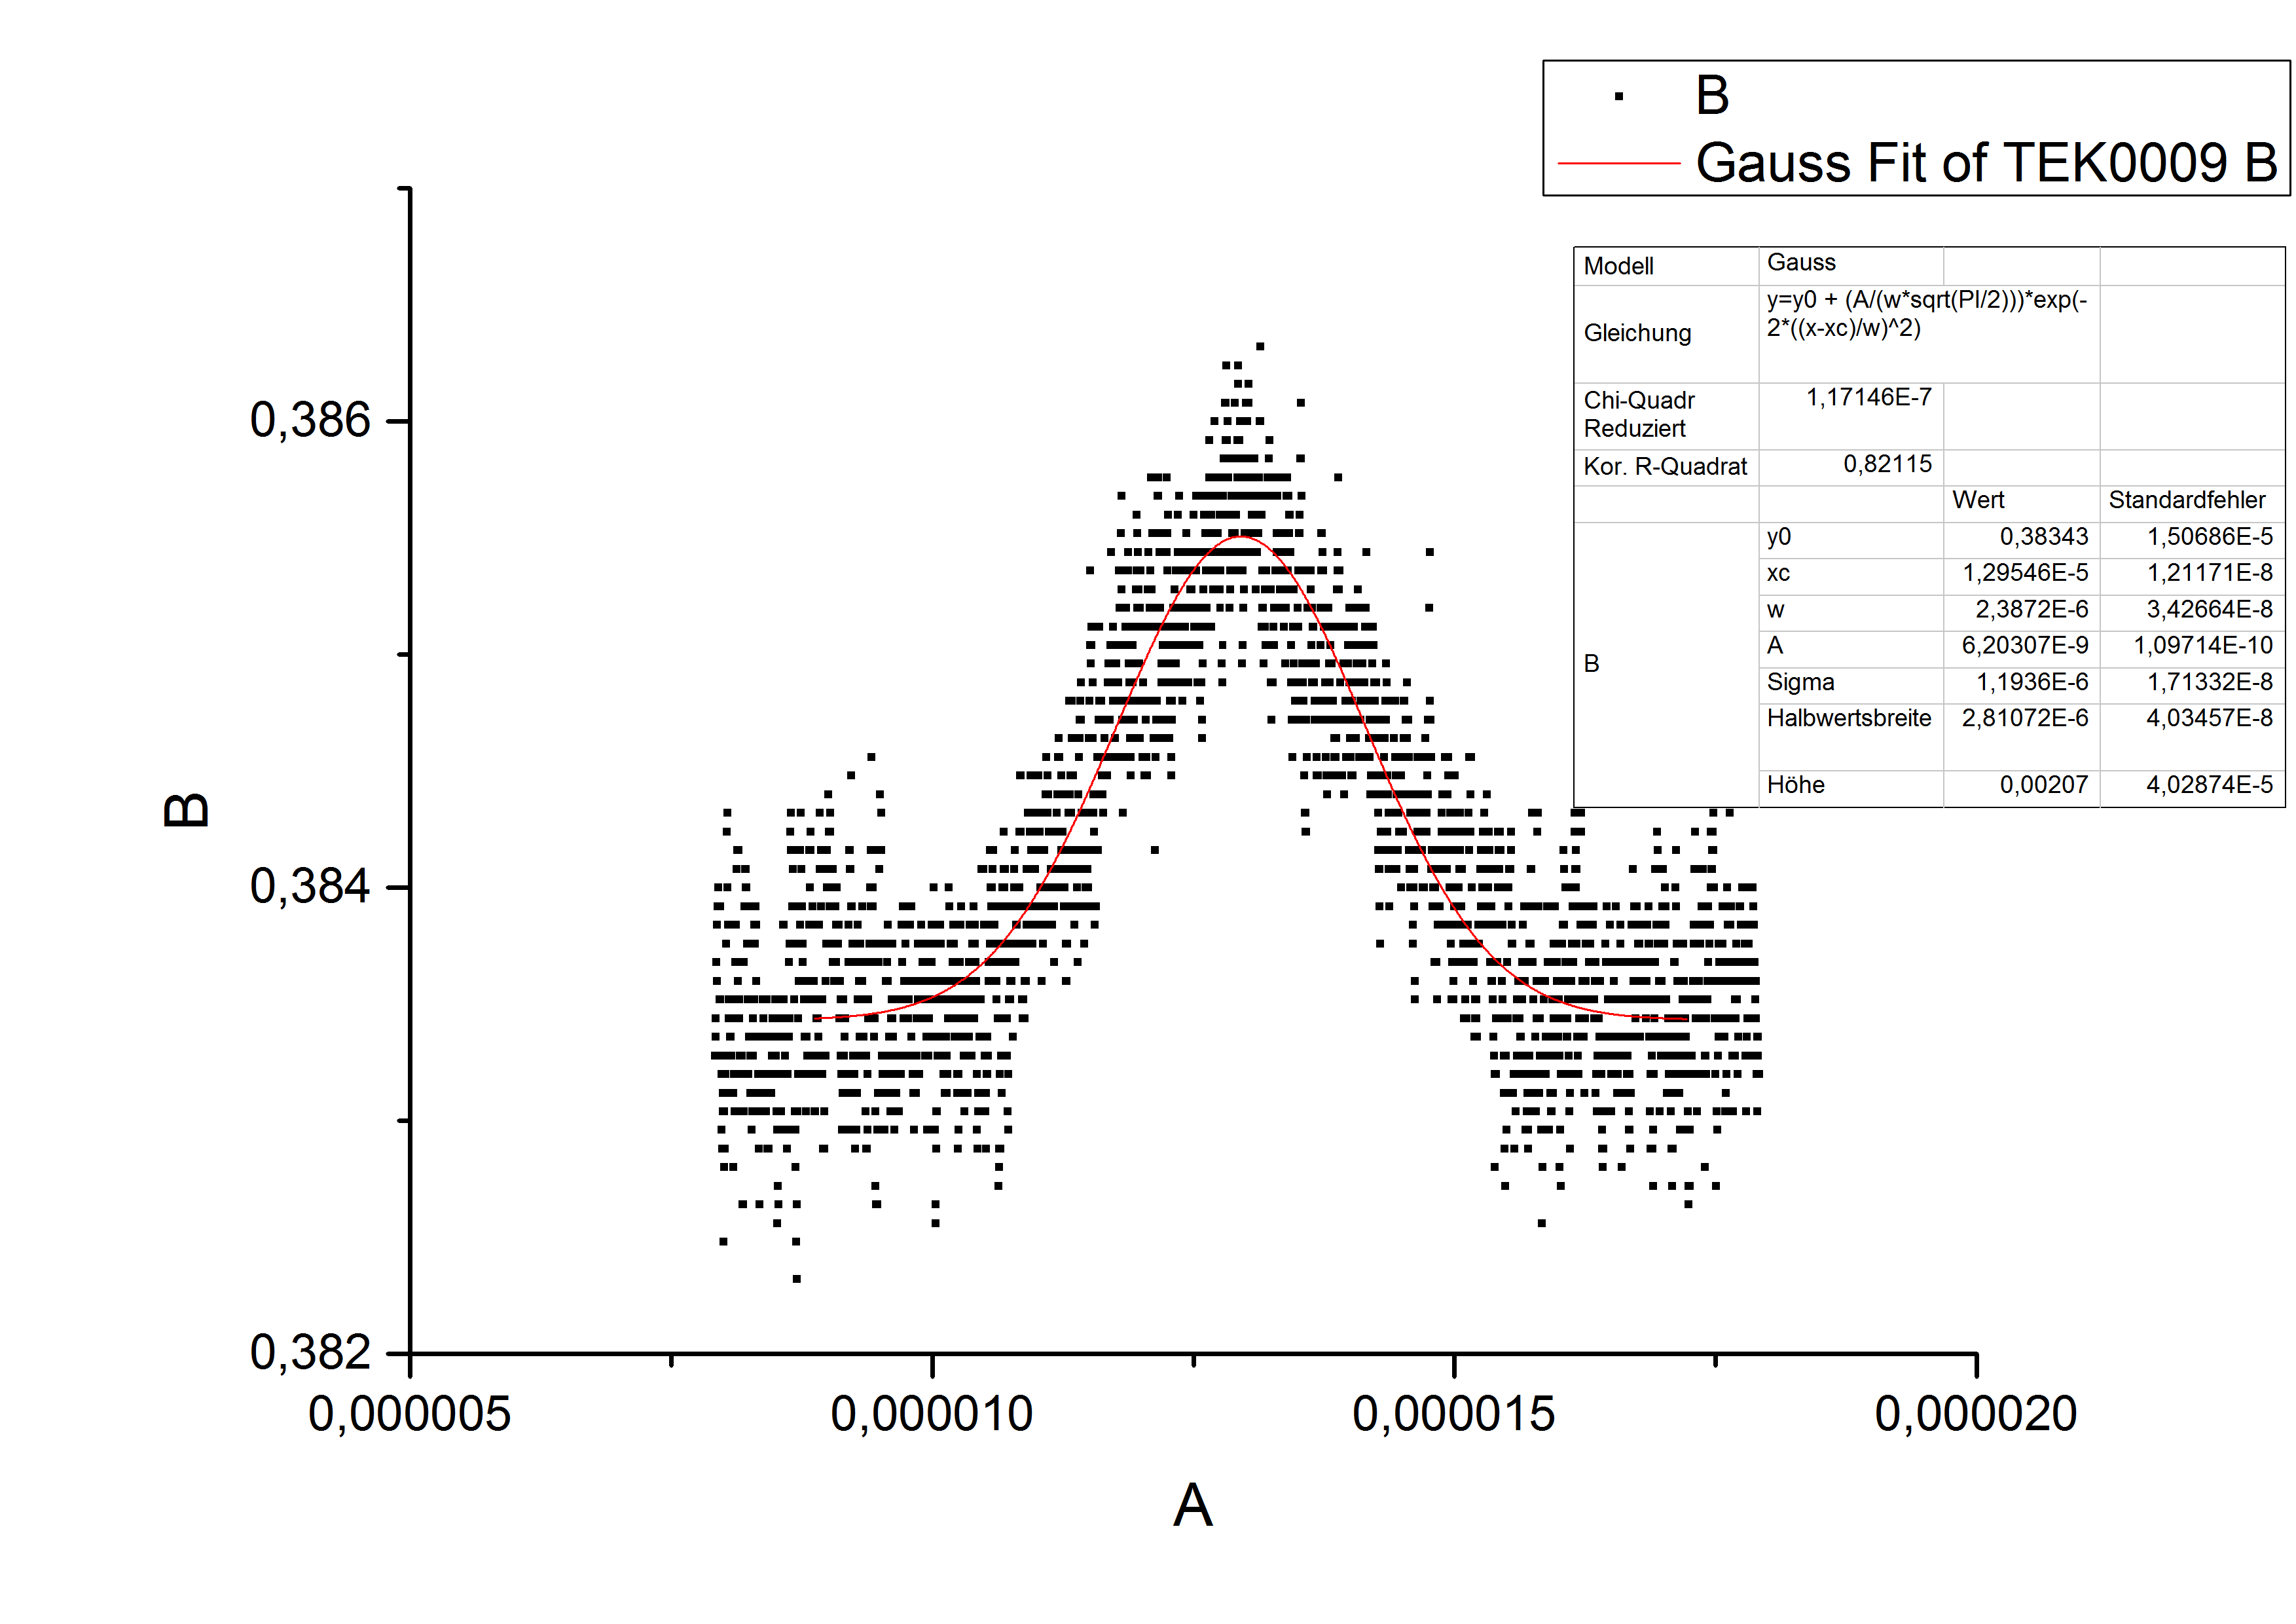
\includegraphics[scale=0.25]{Bilder/Teil2/Graph9}
\caption{Graph at 6.02mm.}
\label{fig:graph9}
\end{center}
\end{figure}
\begin{figure}[h]
\begin{center}
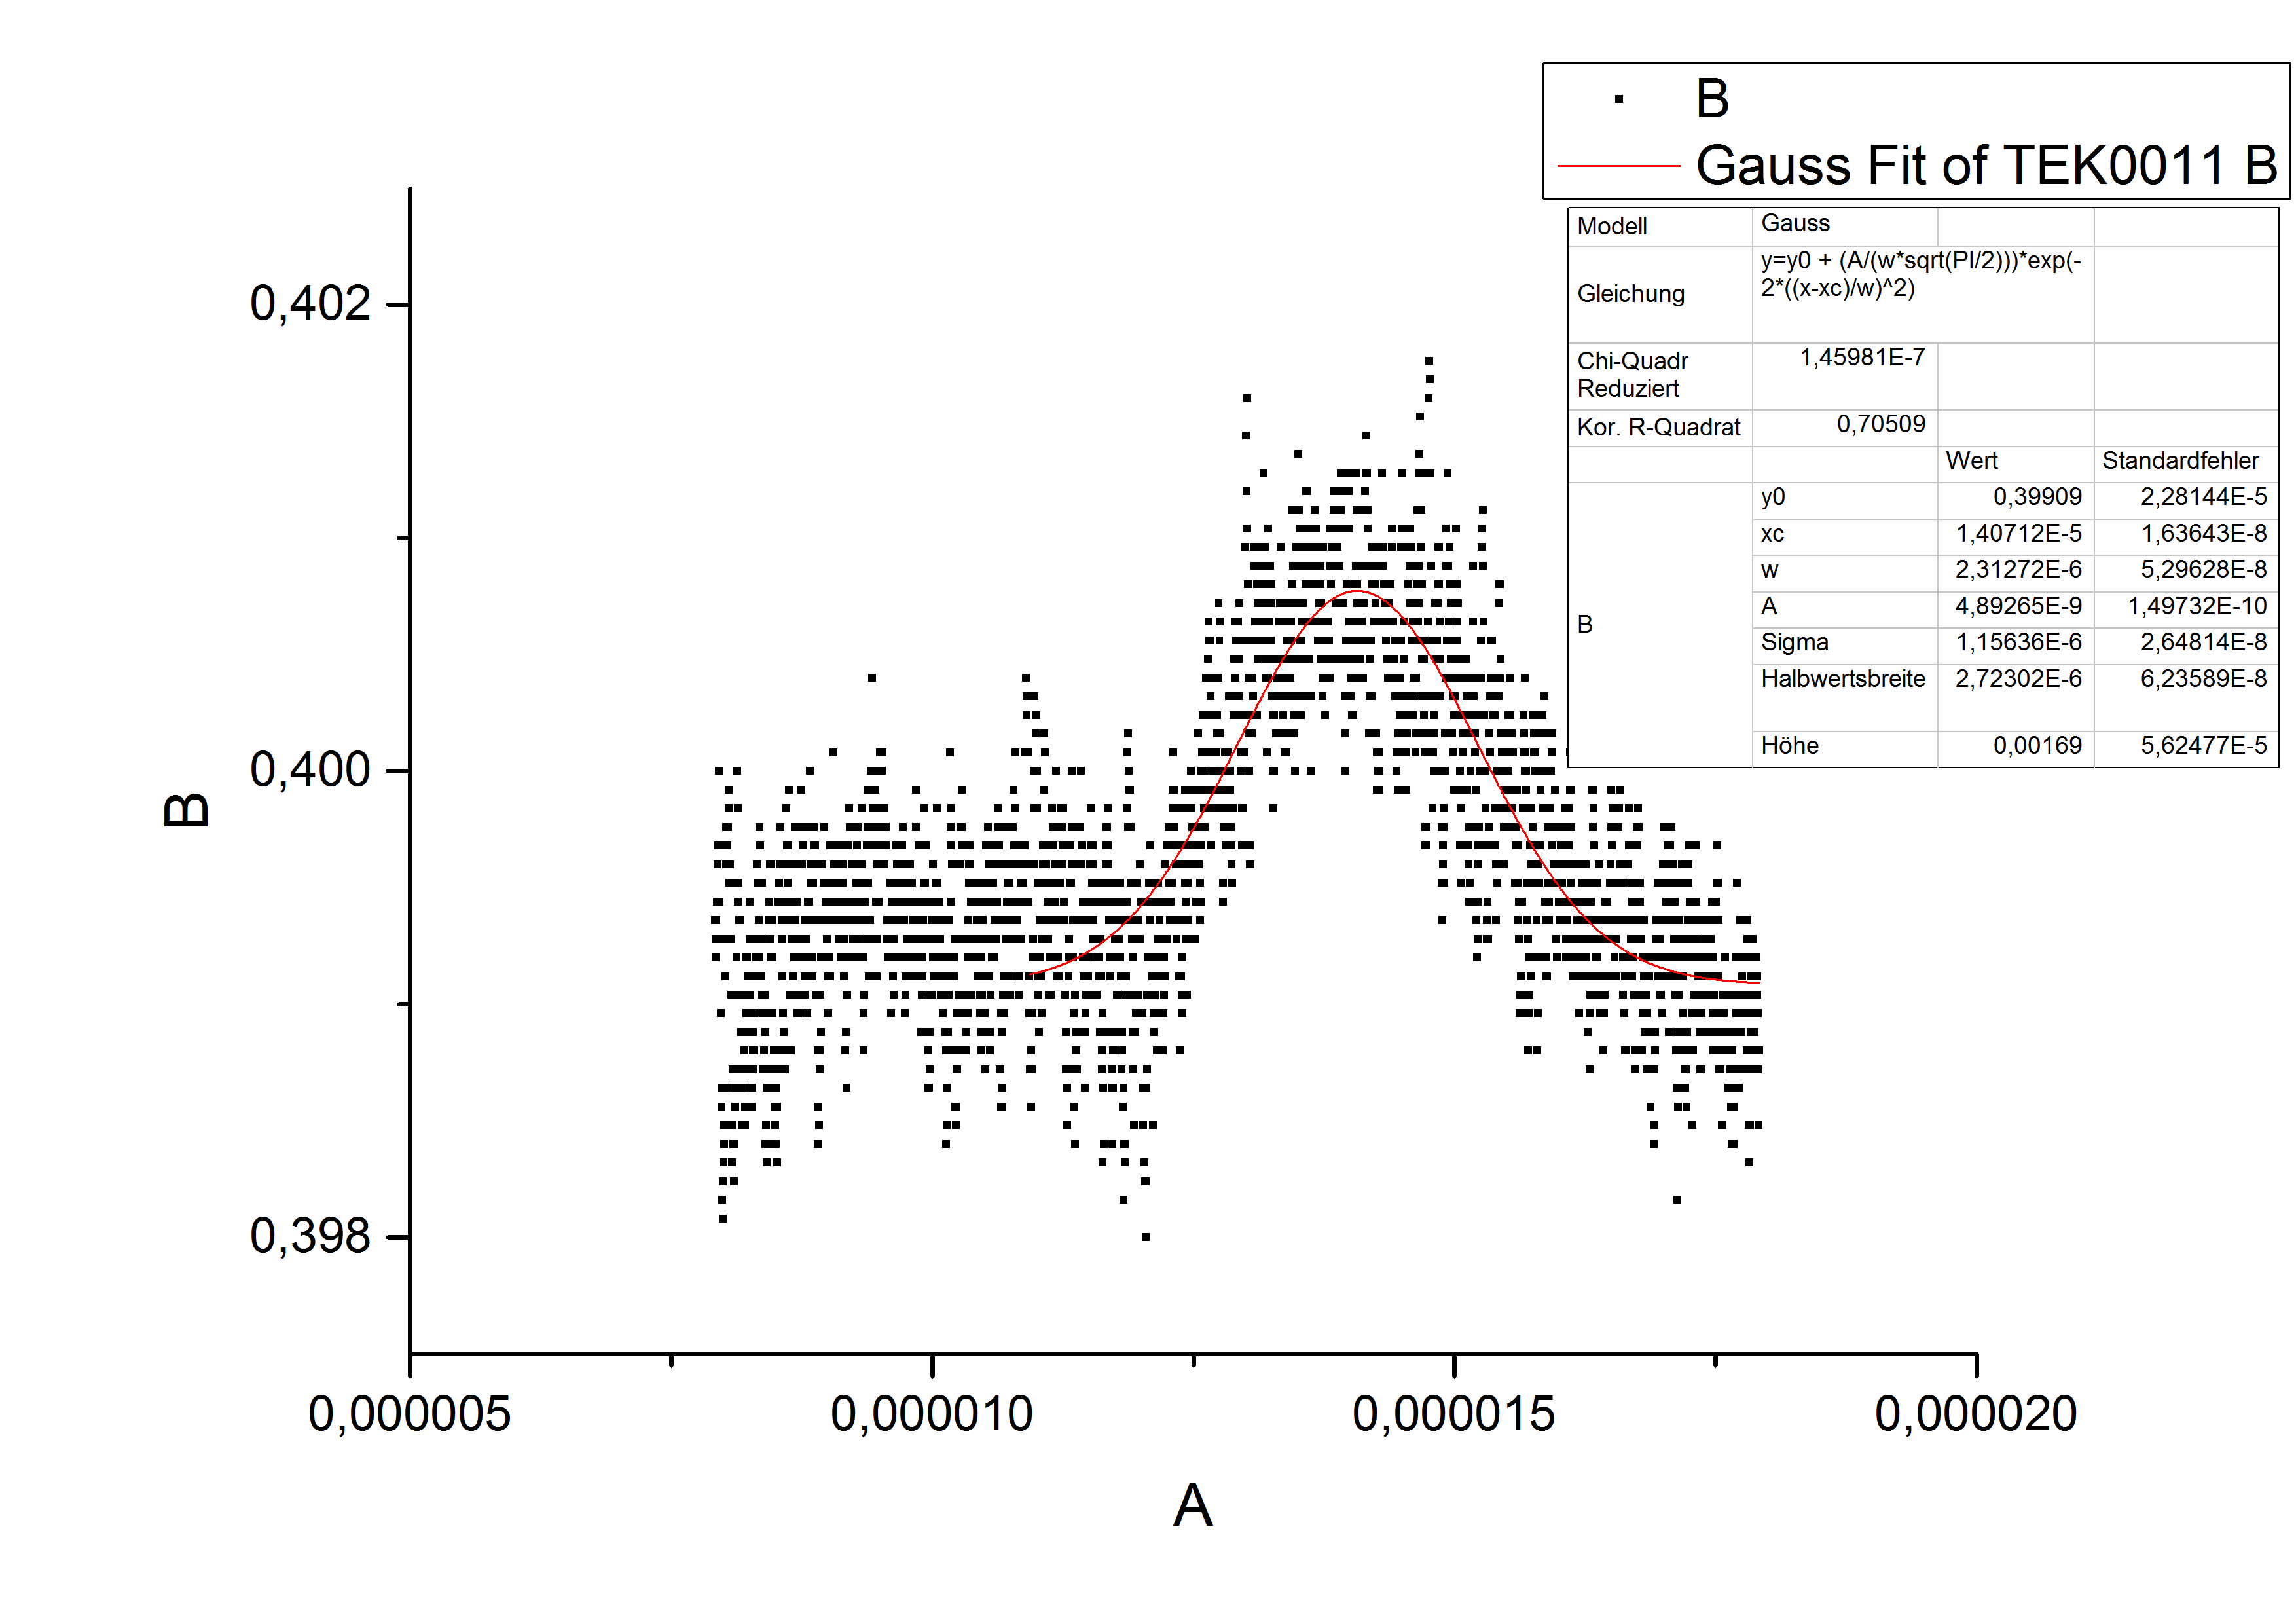
\includegraphics[scale=0.25]{Bilder/Teil2/Graph10}
\caption{Graph at 6.58mm.}
\label{fig:graph10}
\end{center}
\end{figure}
\begin{figure}[h]
\begin{center}
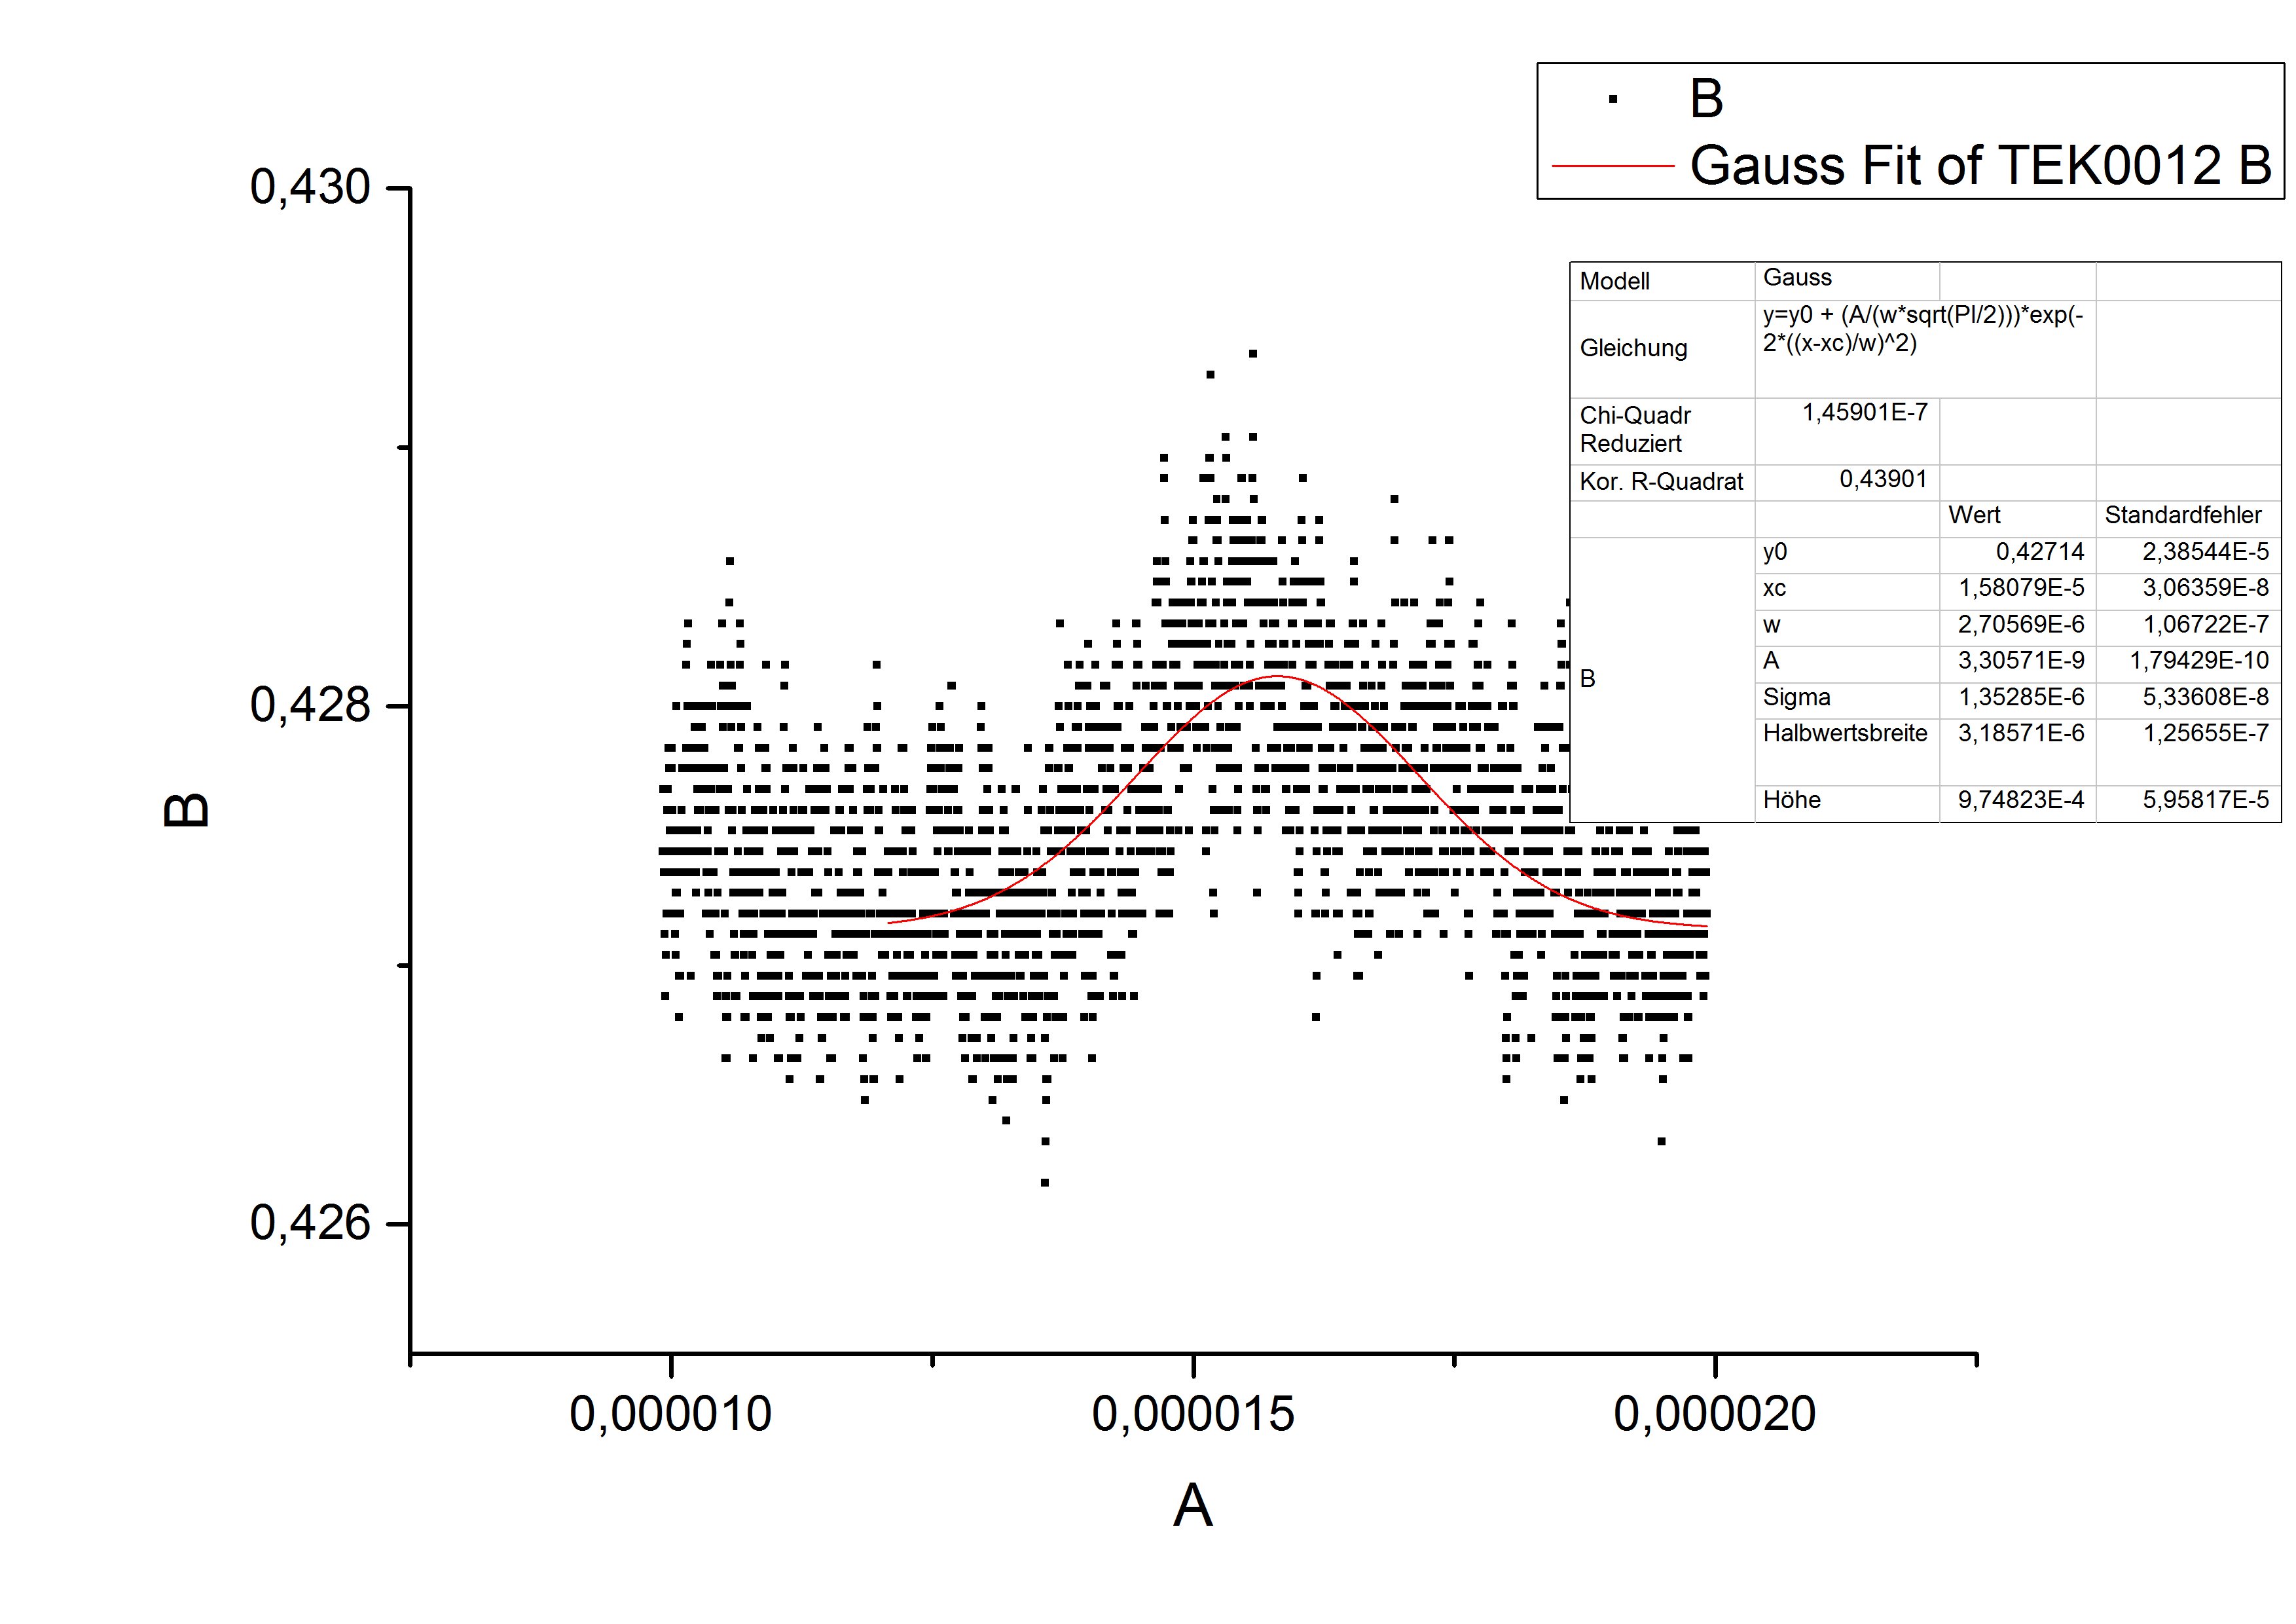
\includegraphics[scale=0.25]{Bilder/Teil2/Graph11}
\caption{Graph at 7.02mm.}
\label{fig:graph11}
\end{center}
\end{figure}
\begin{figure}[h]
\begin{center}
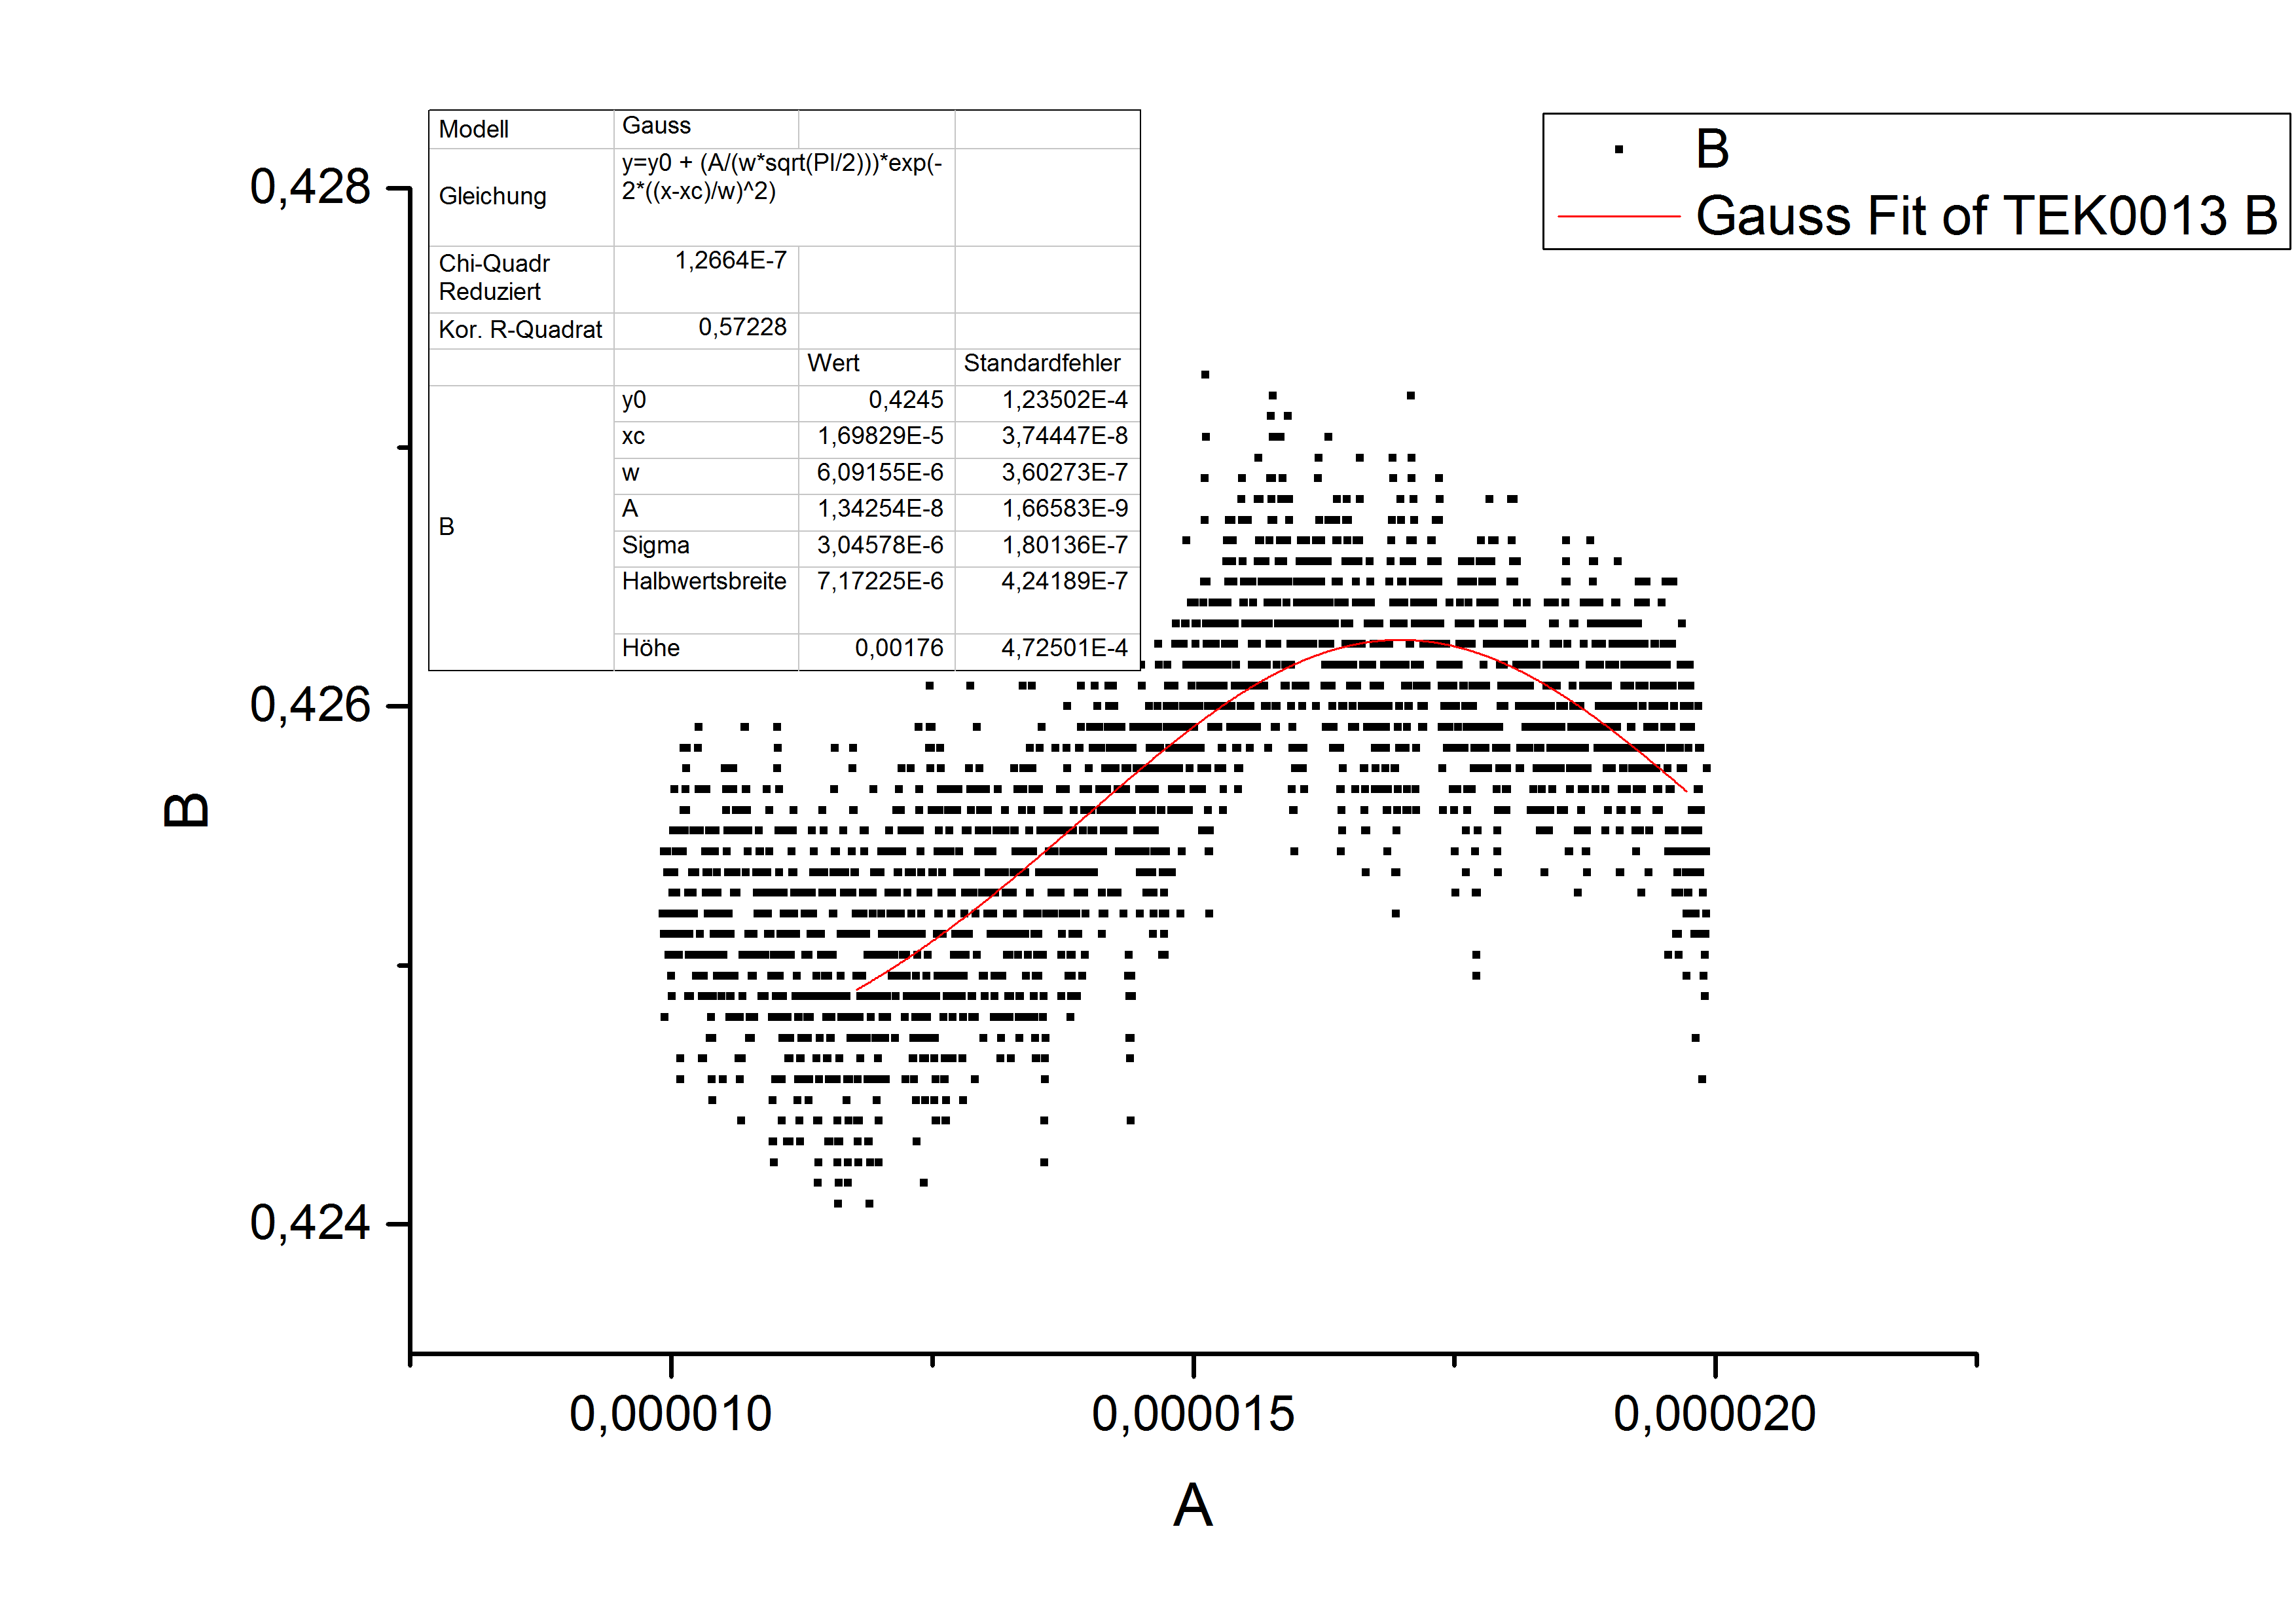
\includegraphics[scale=0.25]{Bilder/Teil2/Graph12}
\caption{Graph at 7.59mm.}
\label{fig:graph12}
\end{center}
\end{figure}
\newpage
\subsection*{Second series of measurements}
\begin{figure}[h]
\begin{center}
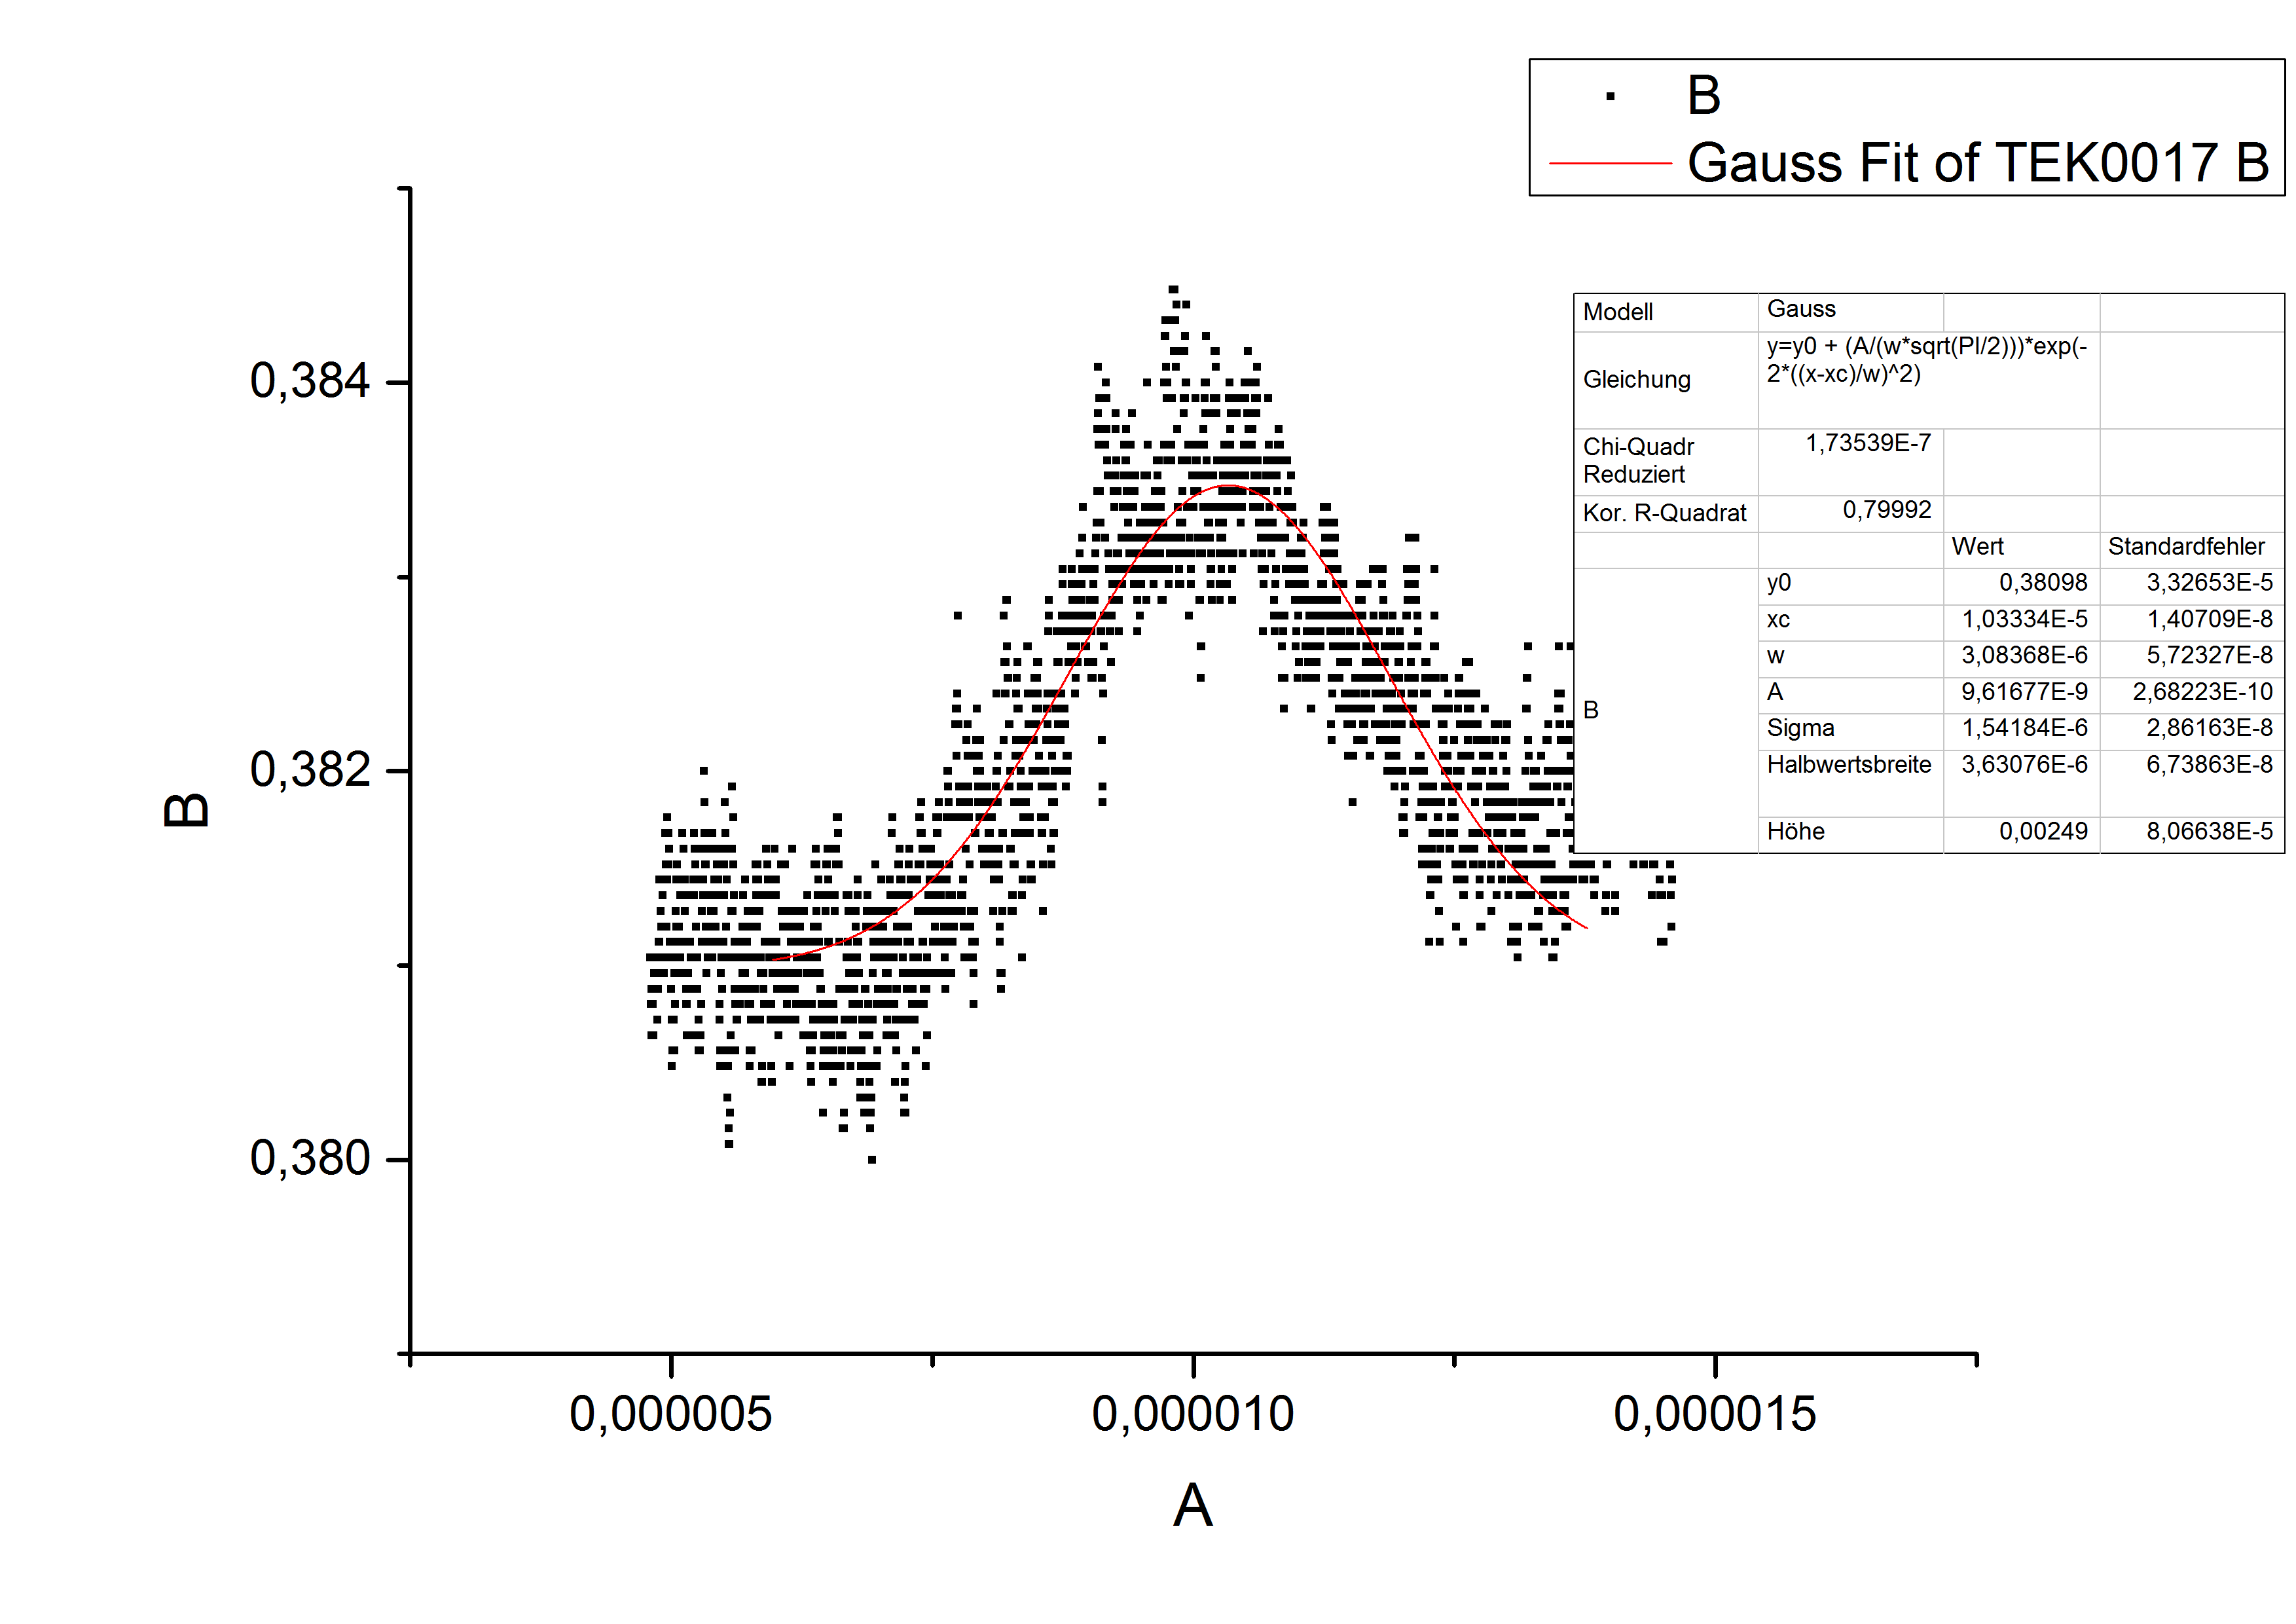
\includegraphics[scale=0.25]{Bilder/Teil2/21}
\caption{Graph at 50V.}
\label{fig:21}
\end{center}
\end{figure}
\begin{figure}[h]
\begin{center}
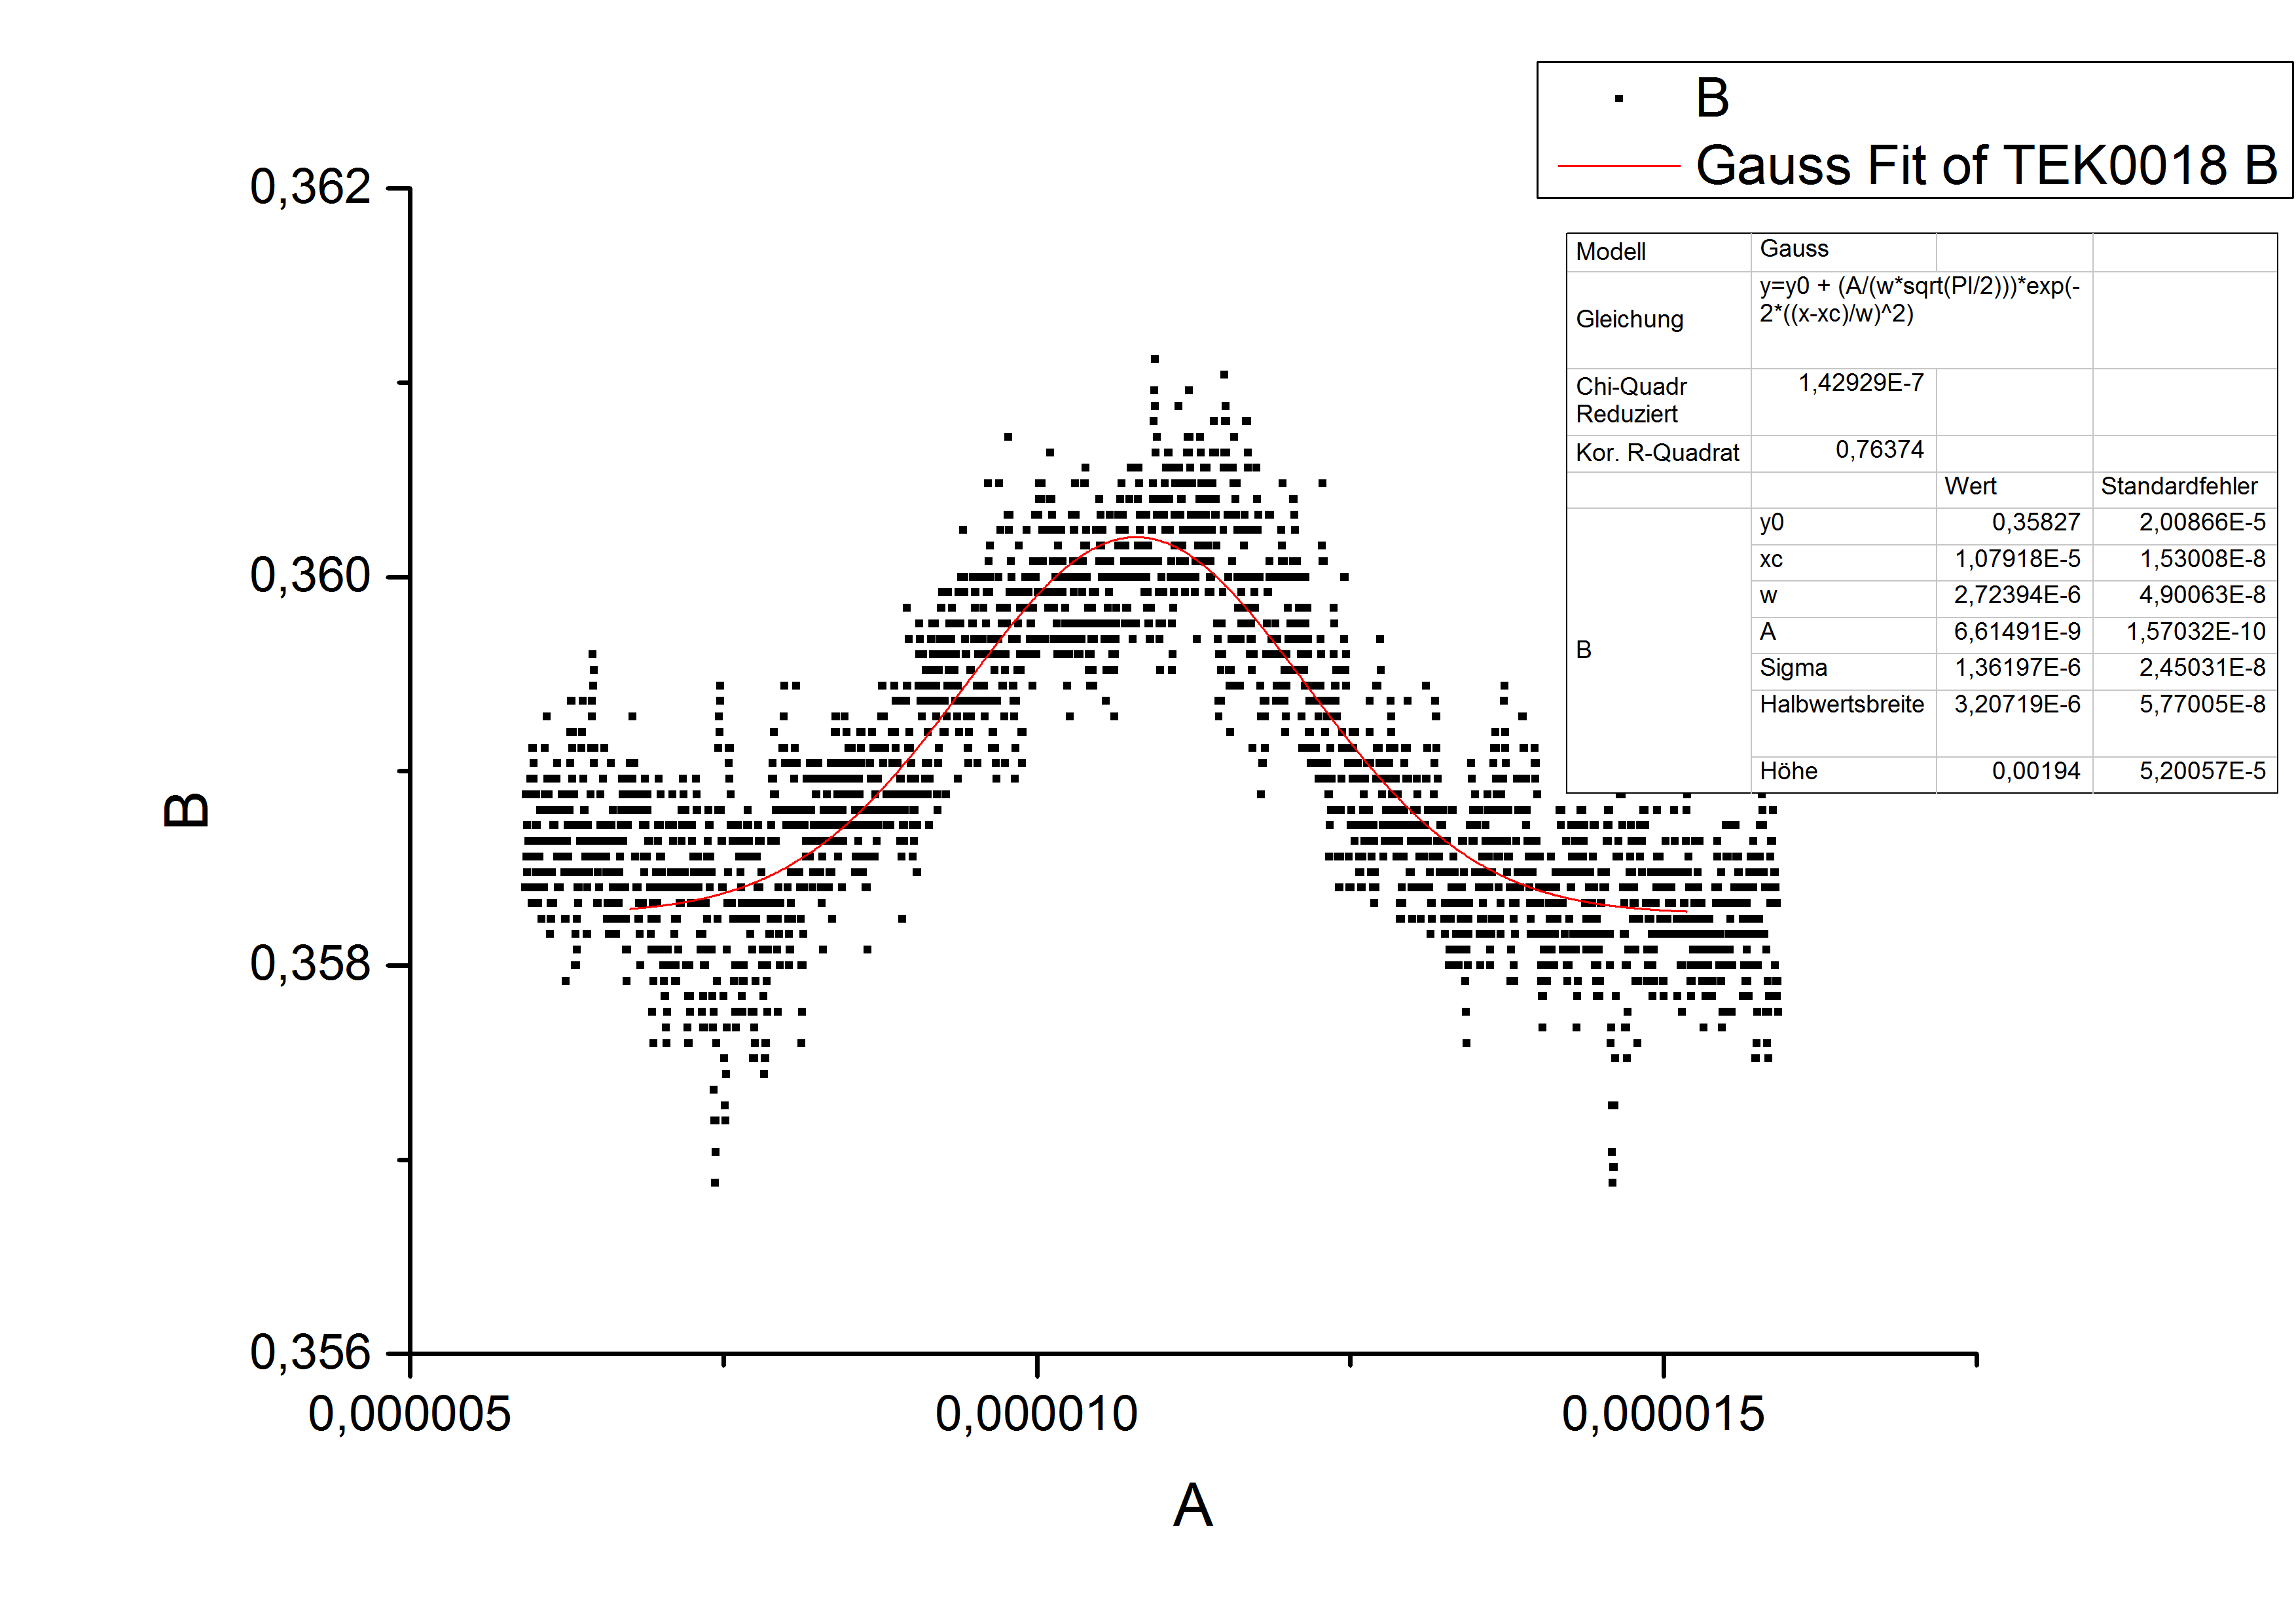
\includegraphics[scale=0.25]{Bilder/Teil2/22}
\caption{Graph at 46V.}
\label{fig:22}
\end{center}
\end{figure}
\begin{figure}[h]
\begin{center}
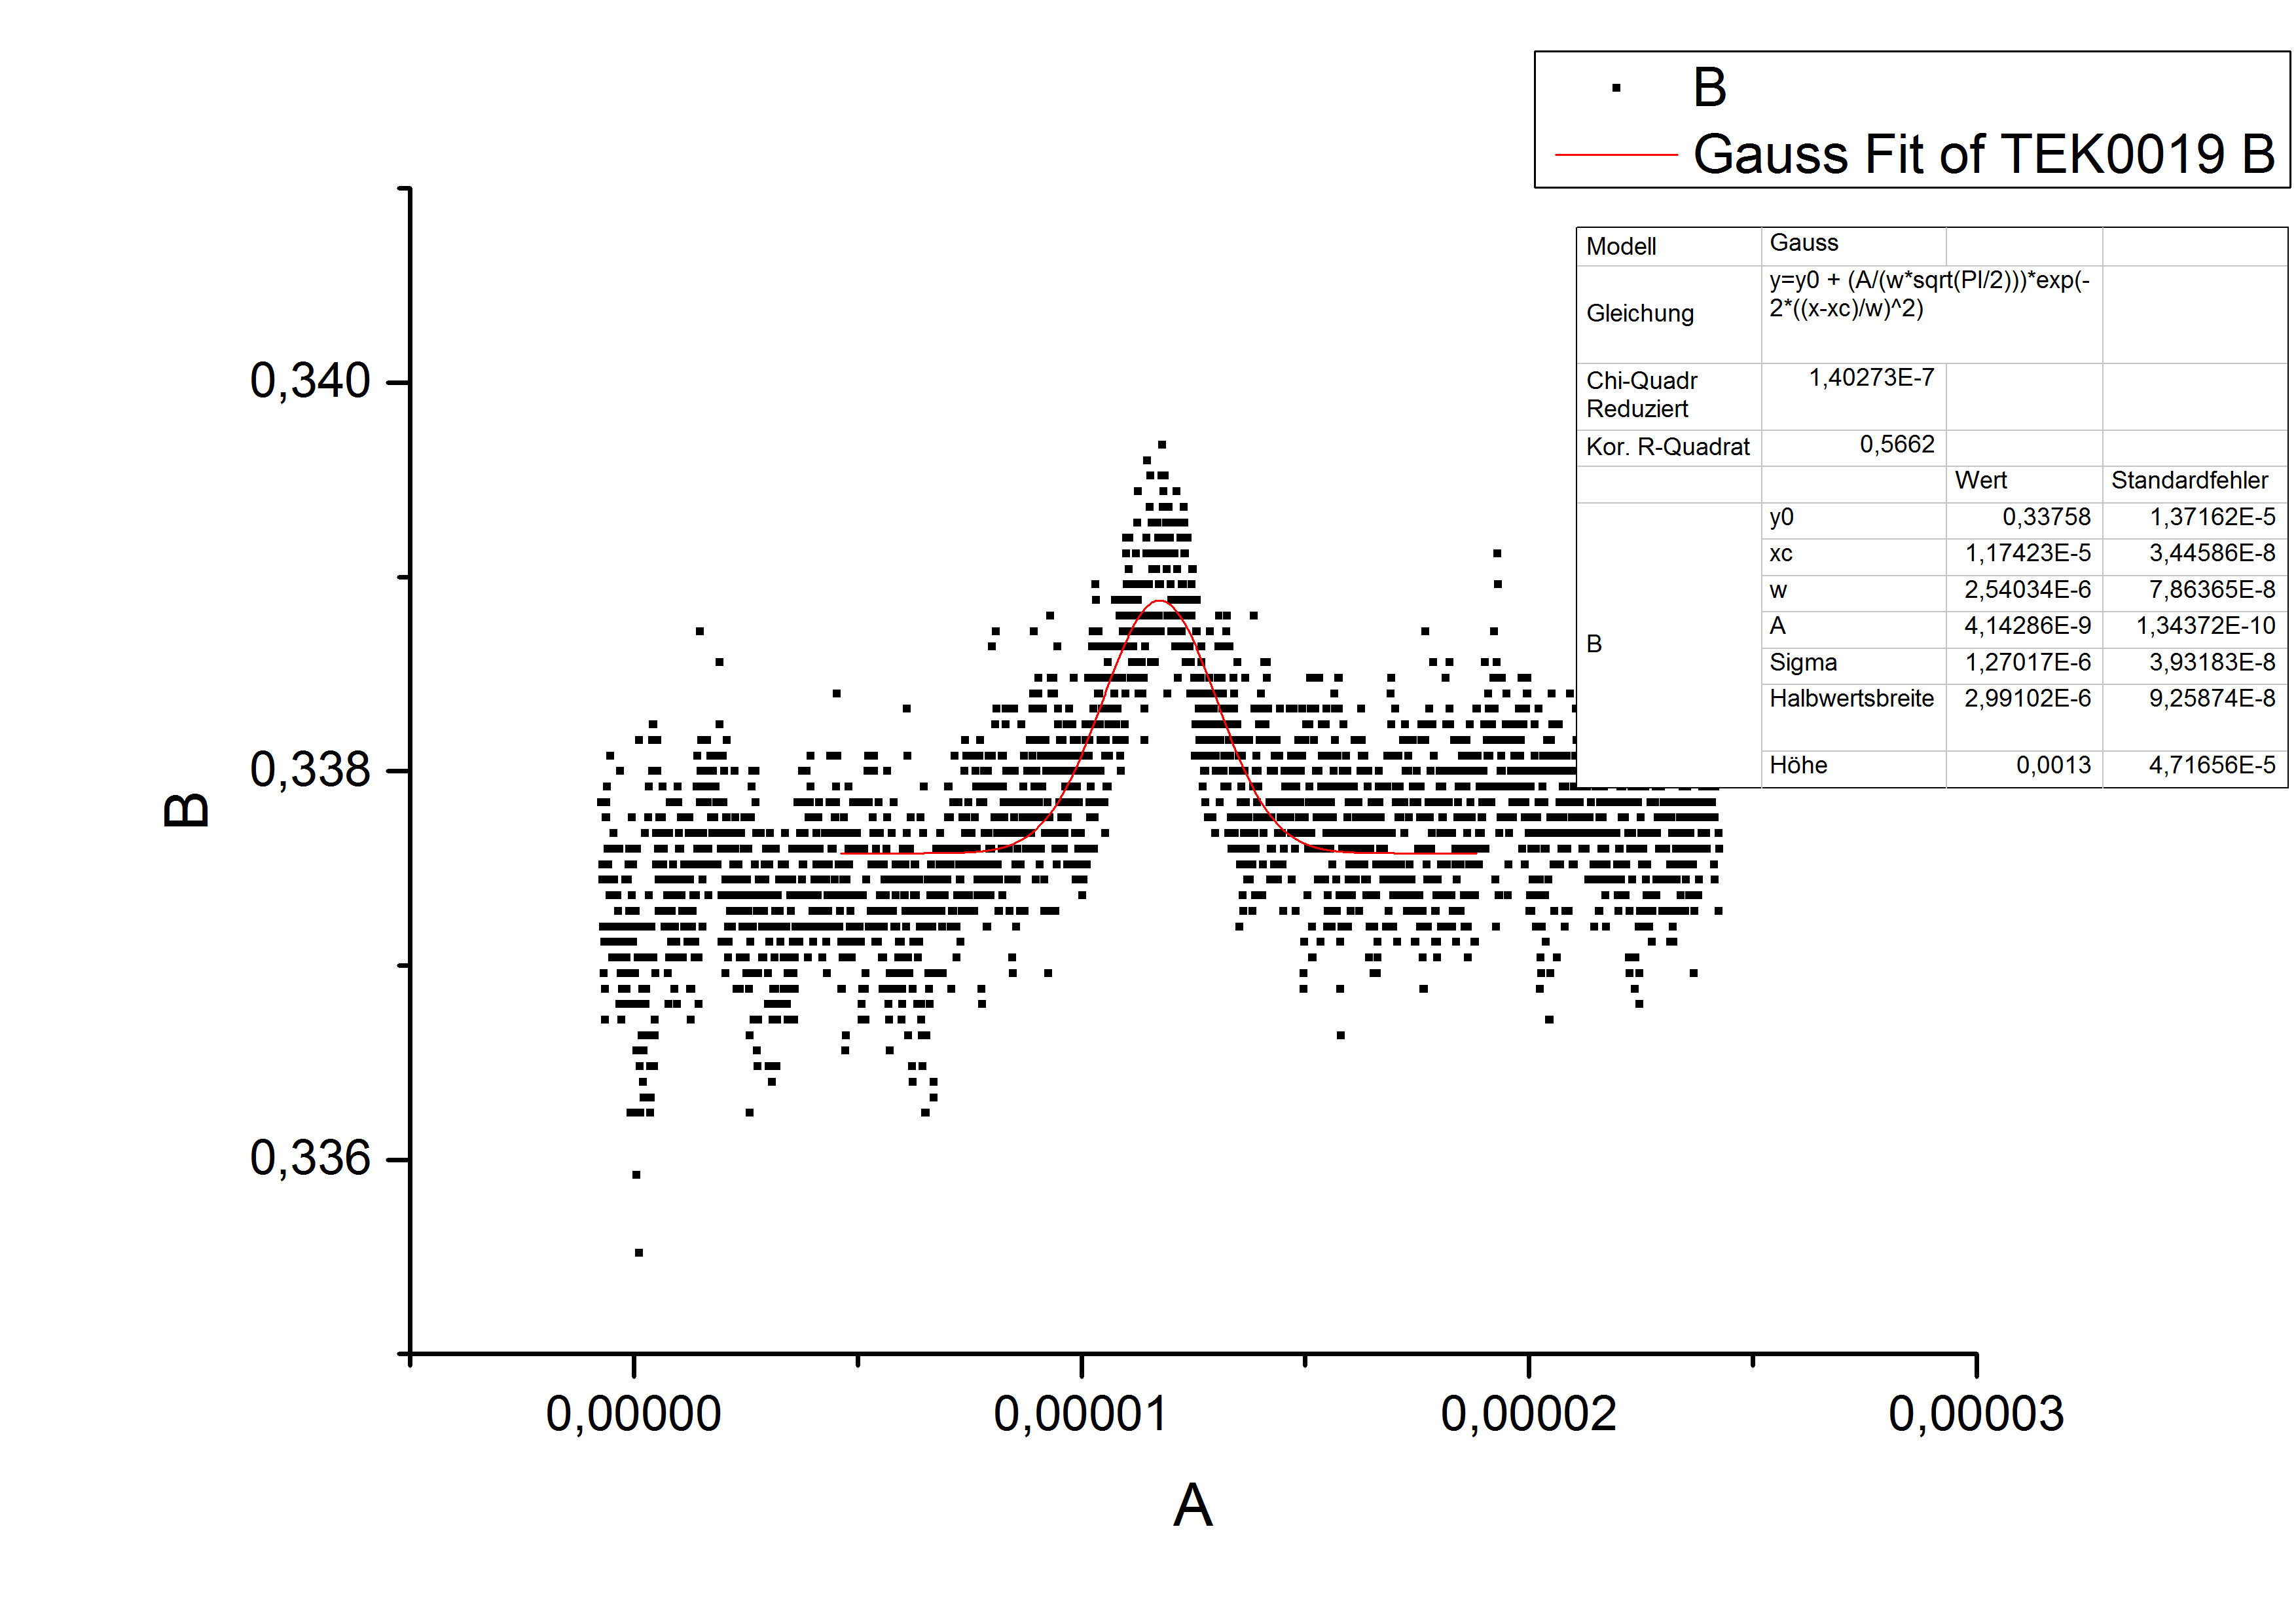
\includegraphics[scale=0.25]{Bilder/Teil2/23}
\caption{Graph at 42V.}
\label{fig:23}
\end{center}
\end{figure}
\begin{figure}[h]
\begin{center}
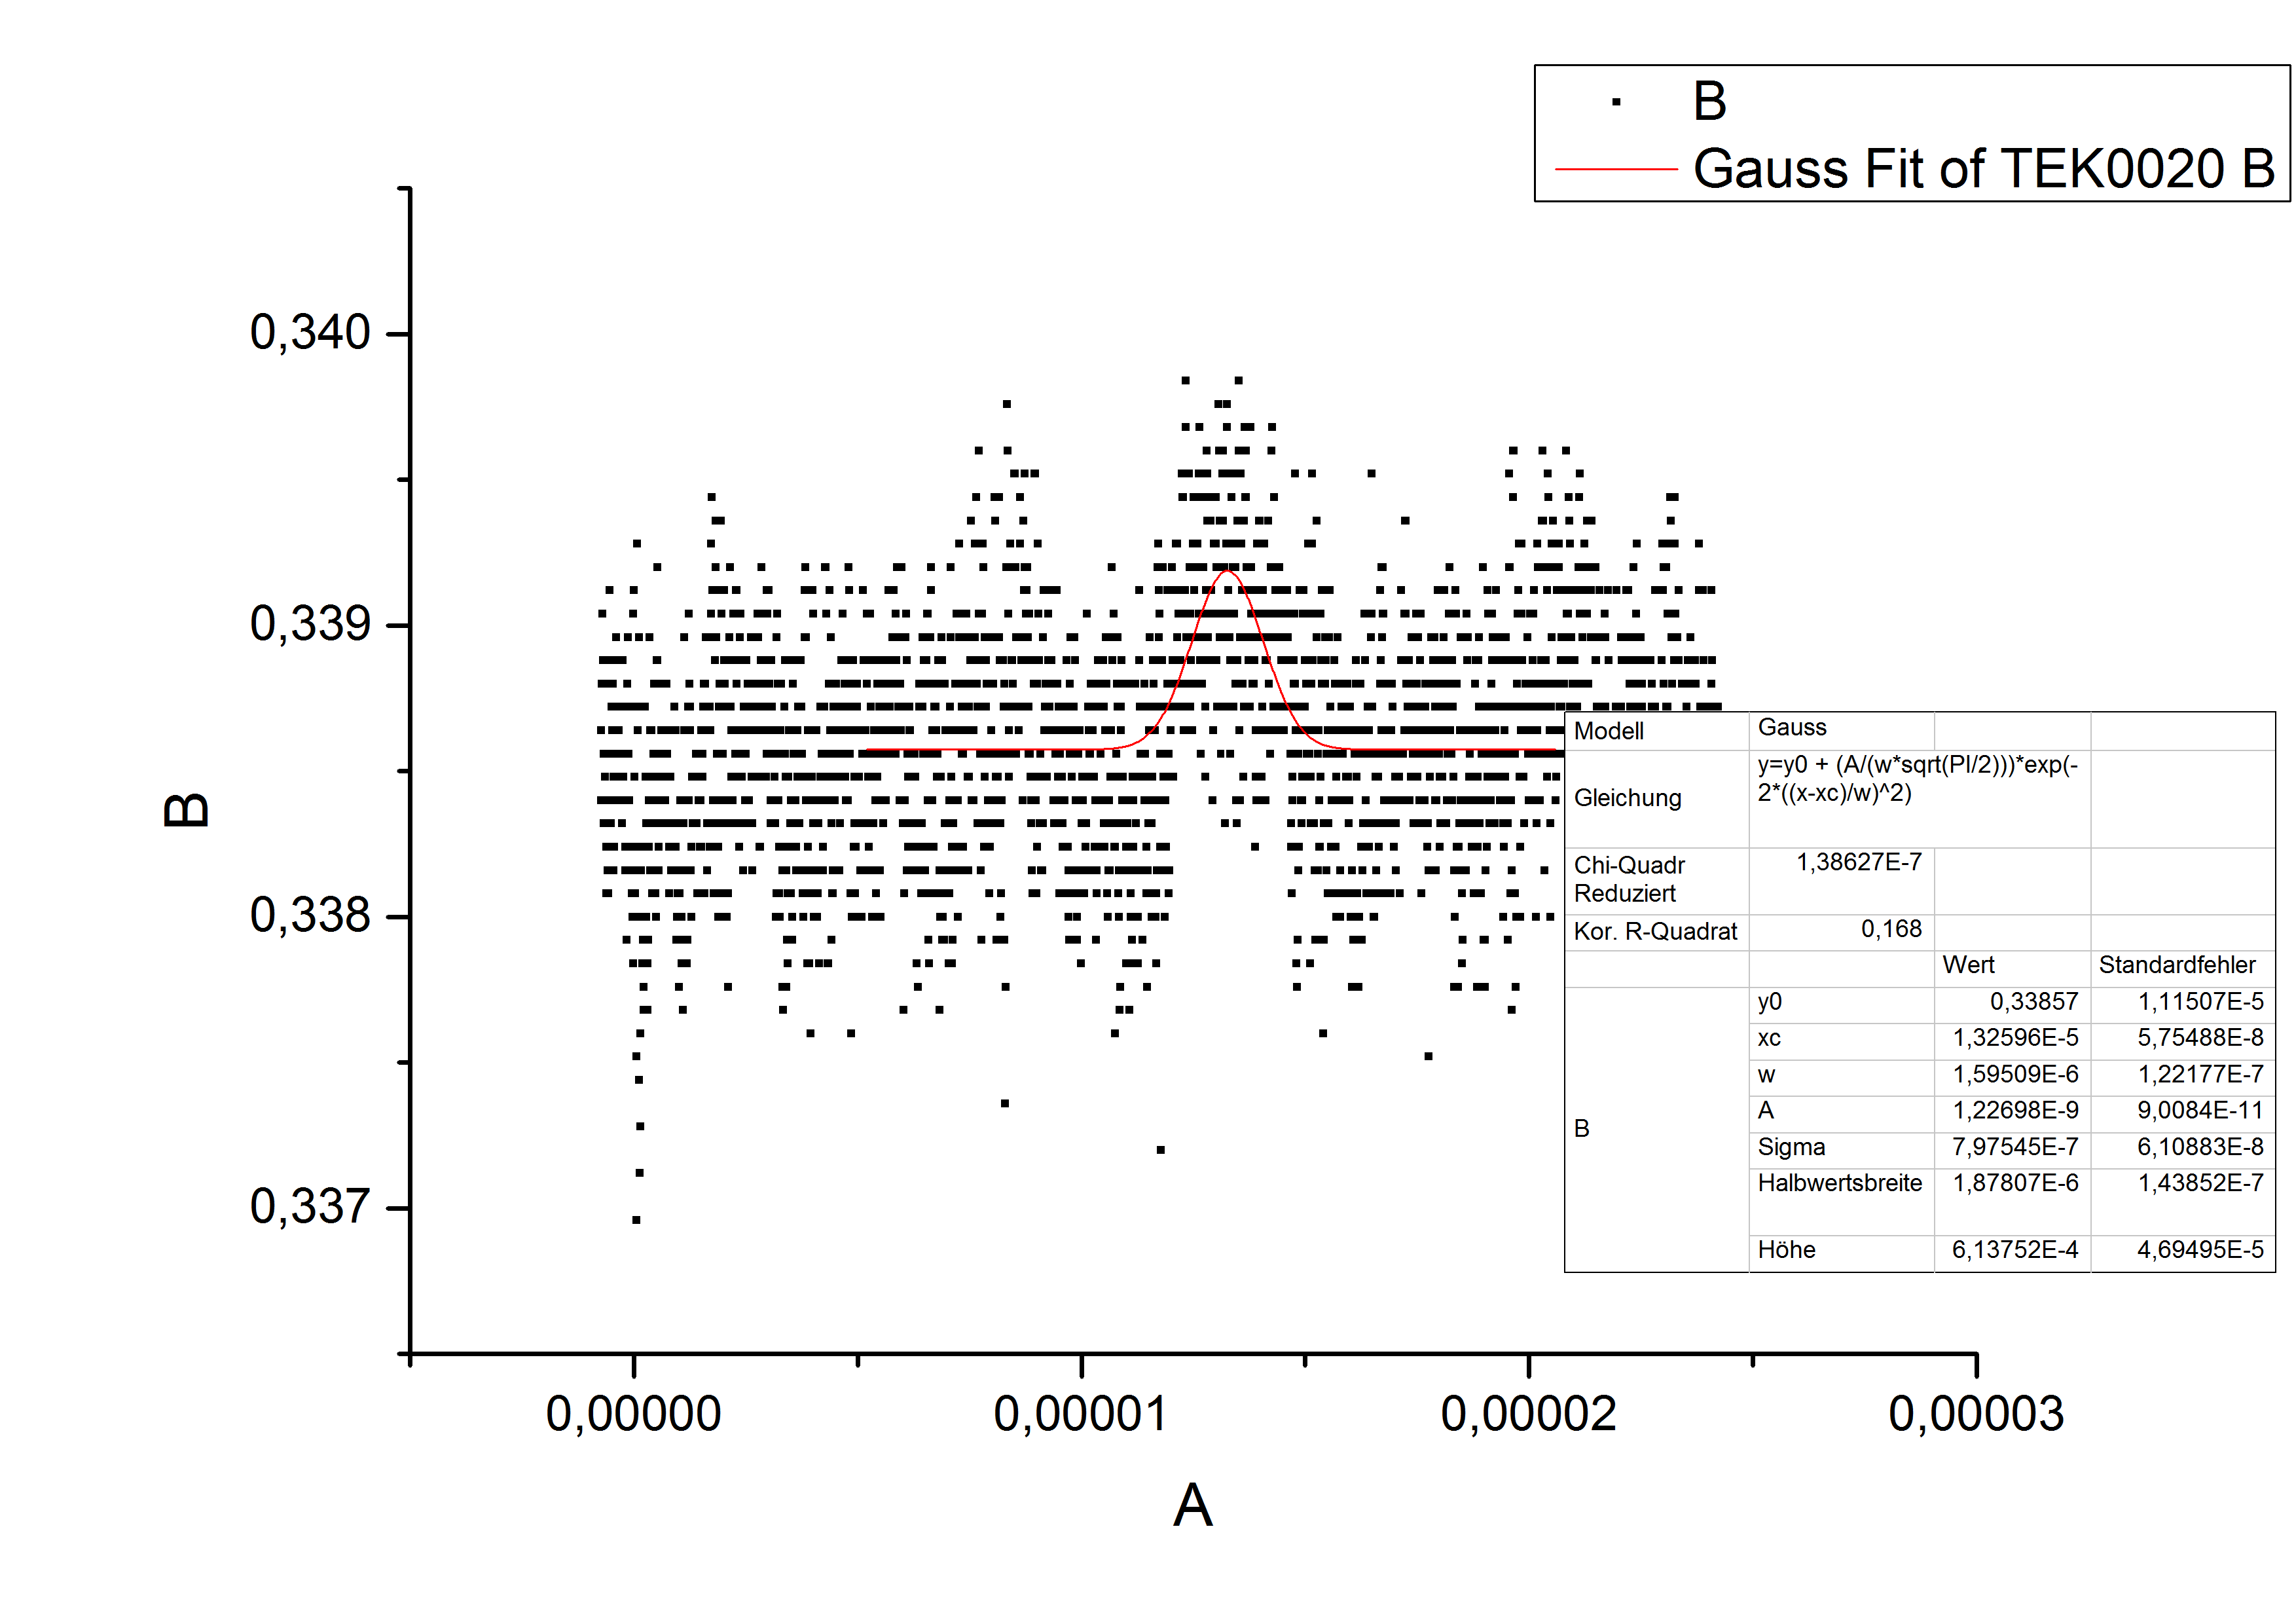
\includegraphics[scale=0.25]{Bilder/Teil2/24}
\caption{Graph 36V.}
\label{fig:24}
\end{center}
\end{figure}
\begin{figure}[h]
\begin{center}
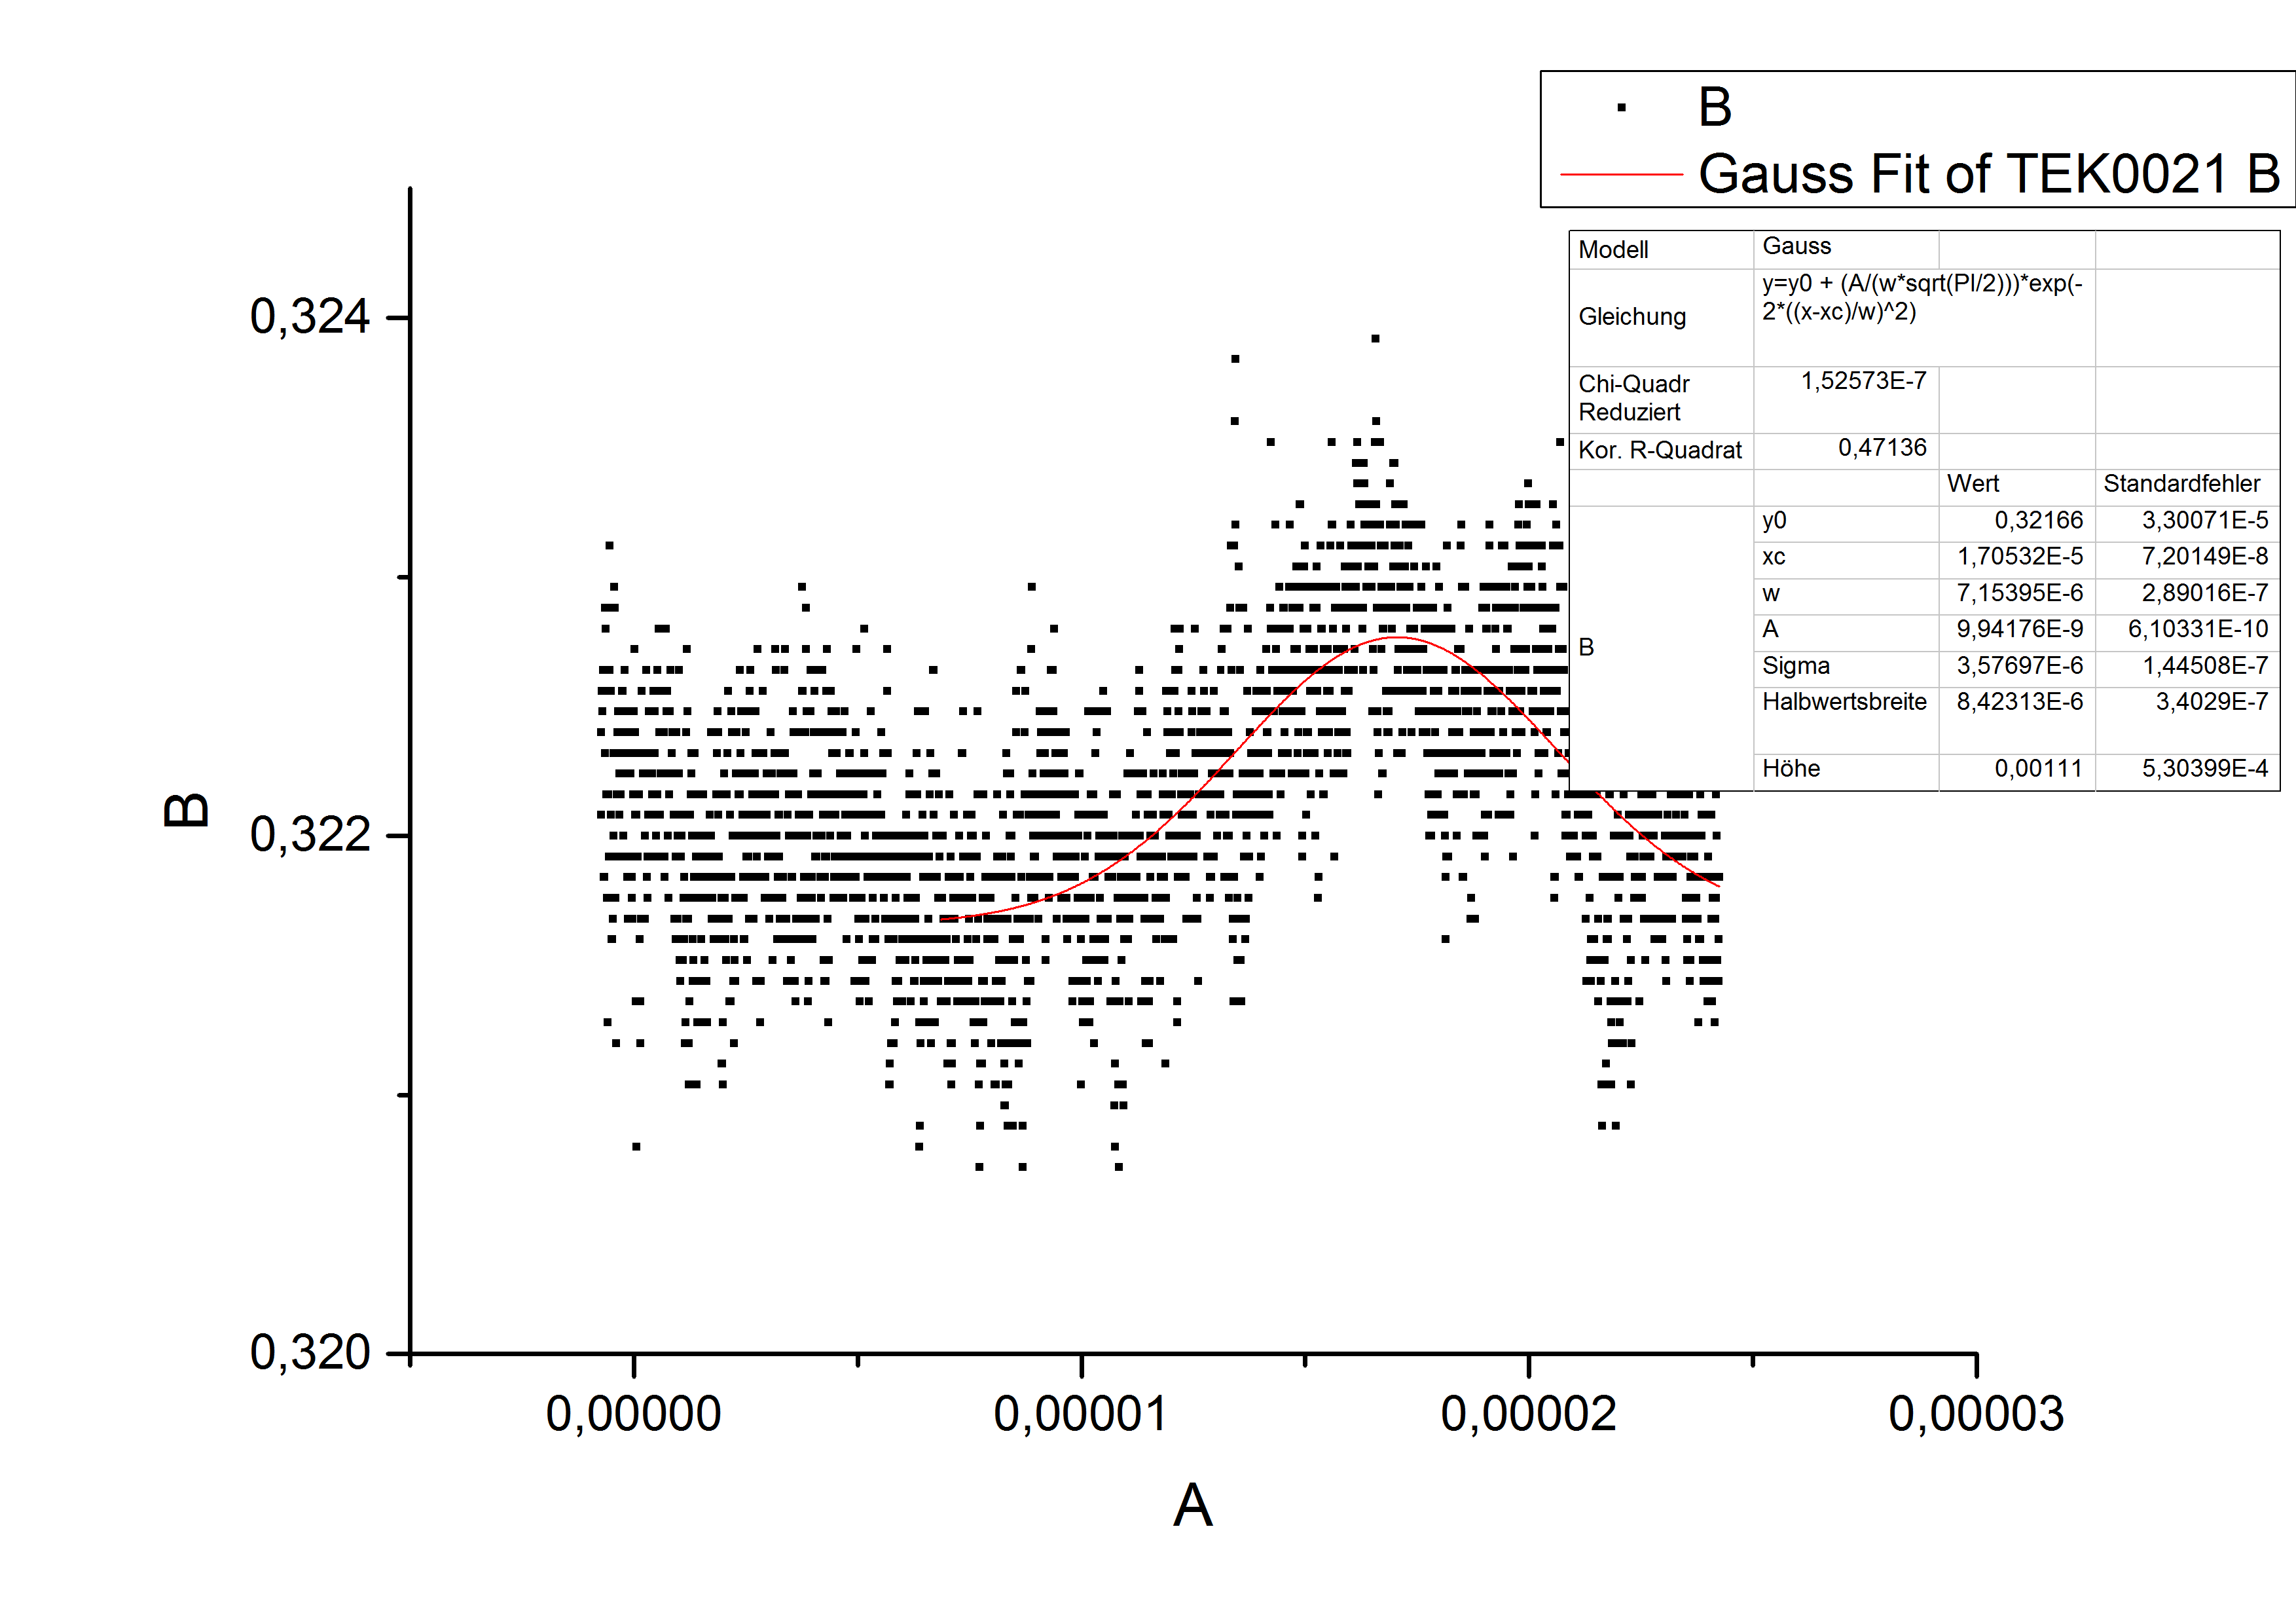
\includegraphics[scale=0.25]{Bilder/Teil2/25}
\caption{Graph 32V.}
\label{fig:25}
\end{center}
\end{figure}
\begin{figure}[h]
\begin{center}
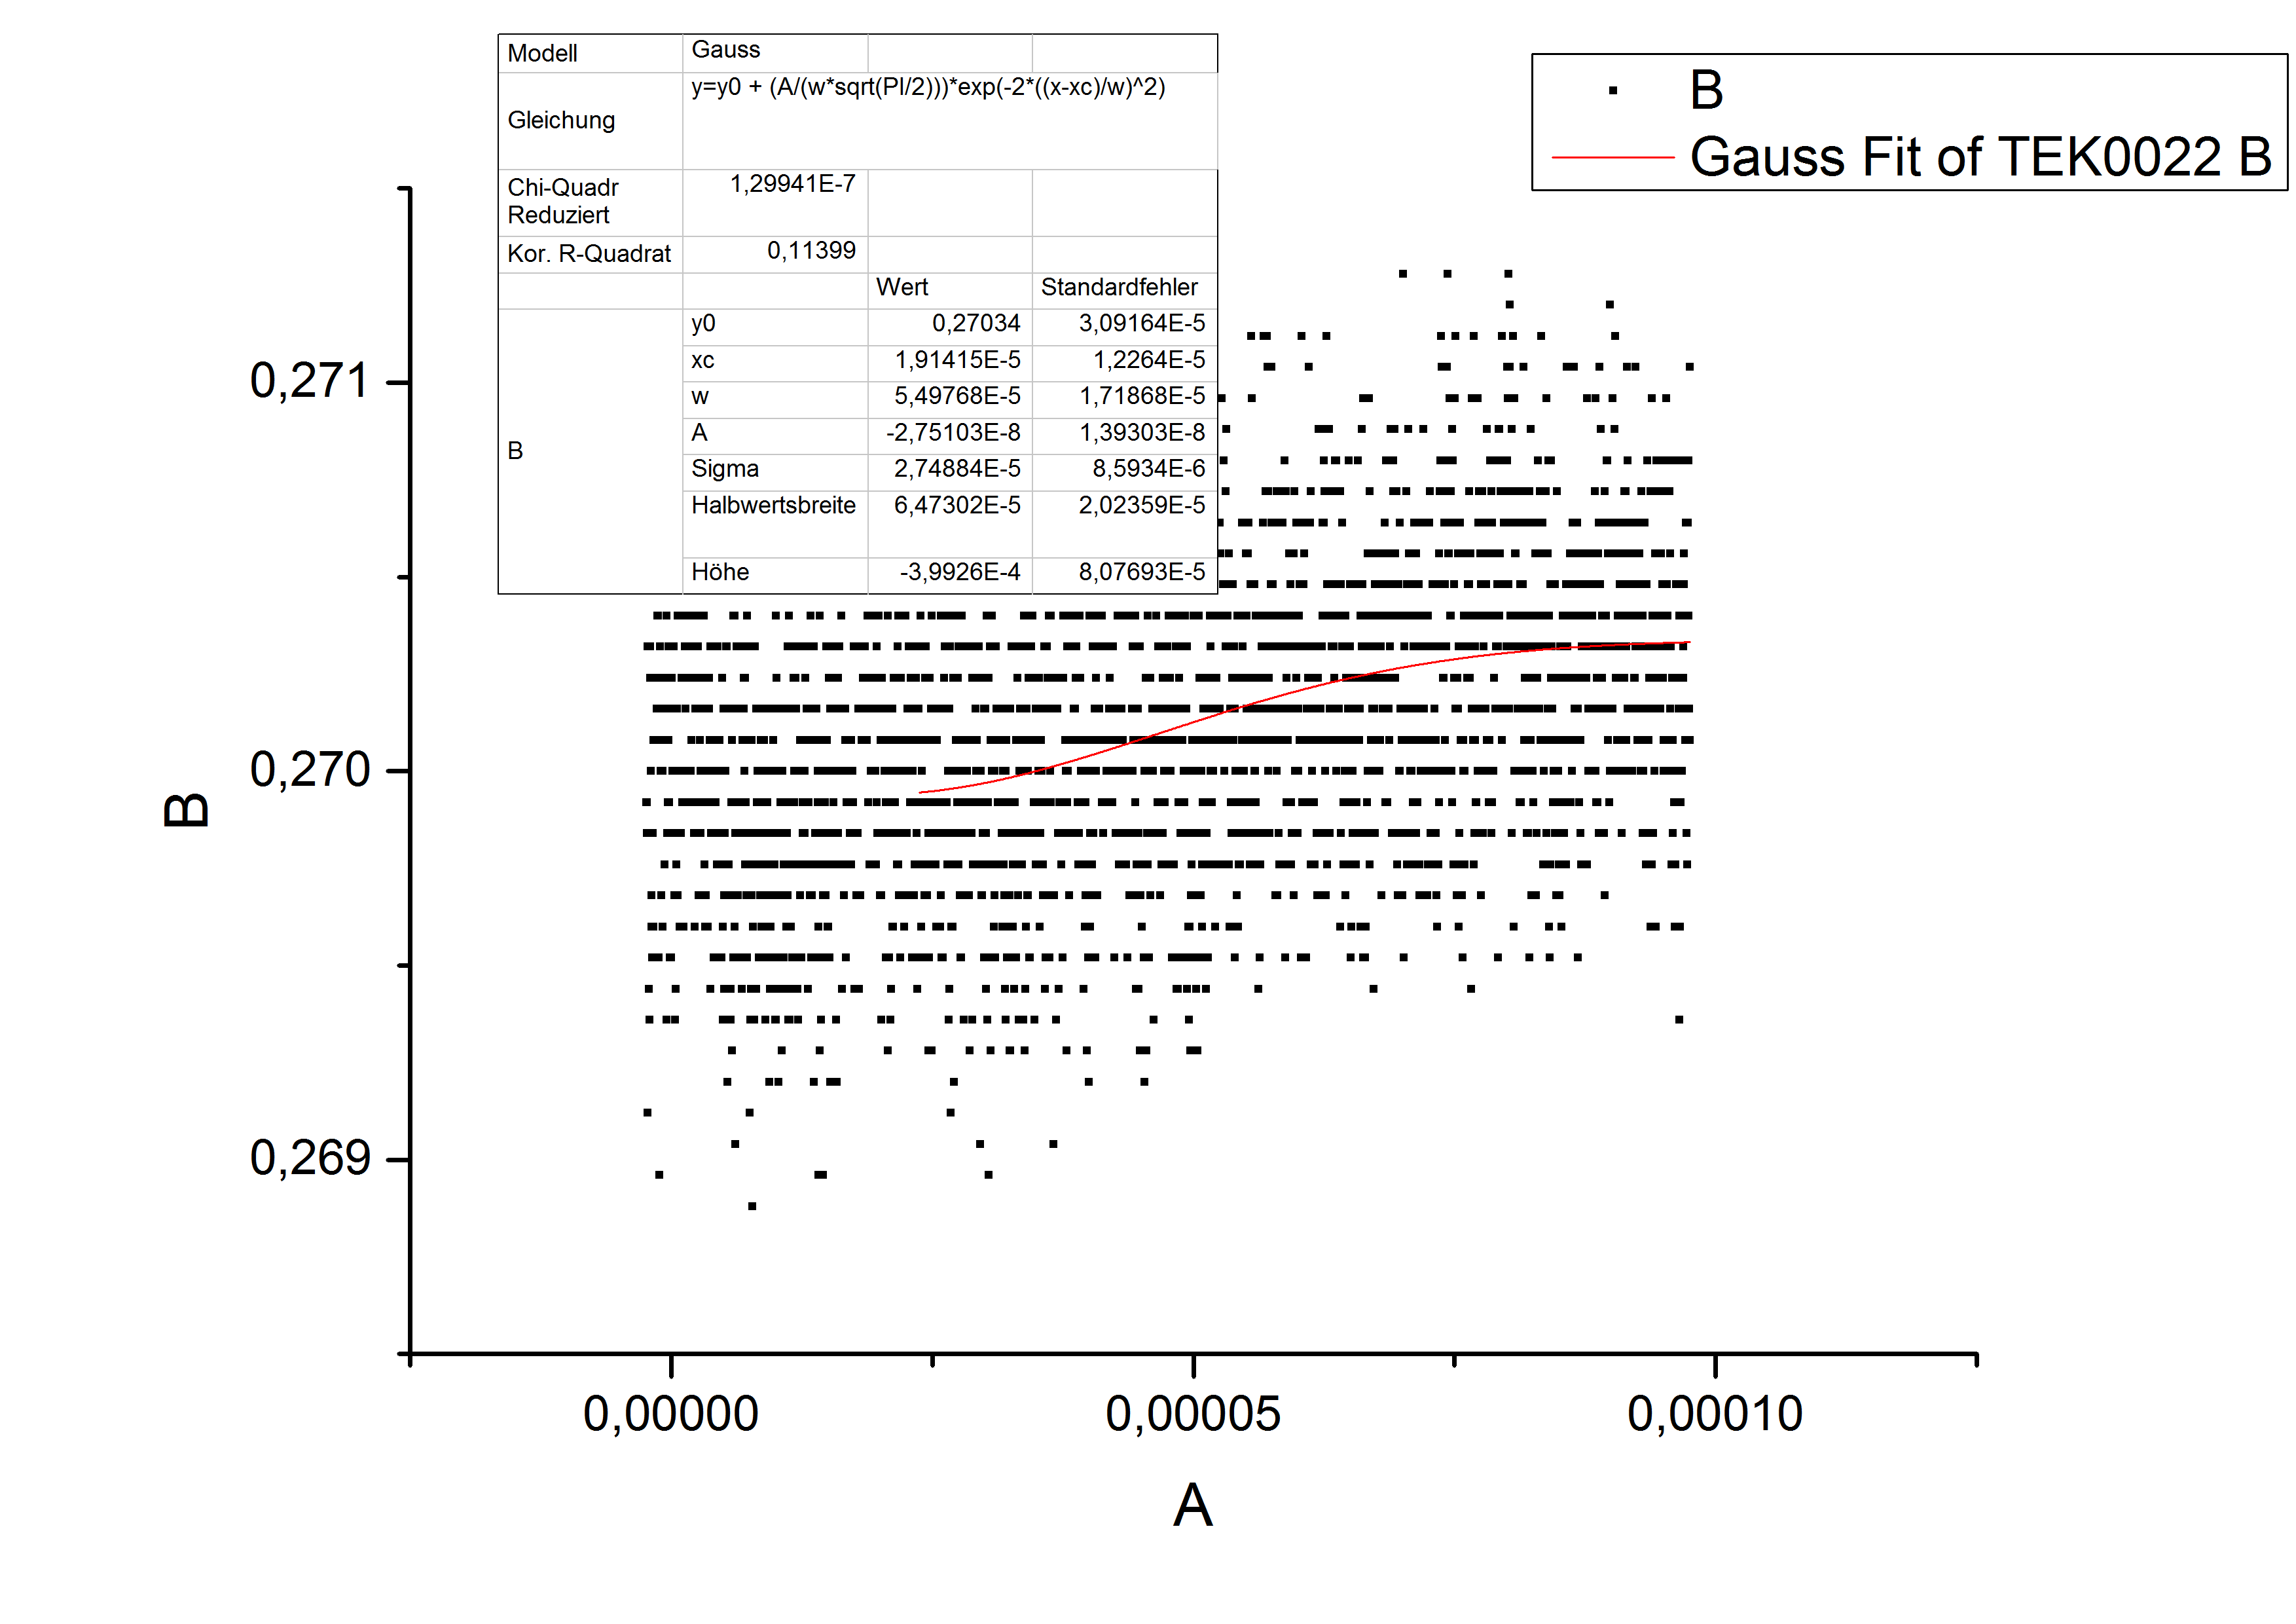
\includegraphics[scale=0.25]{Bilder/Teil2/26}
\caption{Graph 28V.}
\label{fig:26}
\end{center}
\end{figure}